% input files

% document's head

\begin{center}
    \LARGE \textsc{Теория к курсу <<Аналитическая механика II>> ФОПФ}
\end{center}

\hrule

\phantom{42}

\begin{flushright}
    \begin{tabular}{rr}
    % written by:
        \textbf{За авторством}: 
        & Хоружего К. \\
        & Примака Е. \\
        &\\
    % date:
        \textbf{От}: &
        \textit{\today}\\
    \end{tabular}
\end{flushright}

\thispagestyle{empty}
\tableofcontents
\newpage


% \section{Первое задание по аналитической механике \texorpdfstring{(\checkmark)}{(ок)}}


% \subsection{Малые колебания консервативных систем \texorpdfstring{(\checkmark)}{(ок)}}
% \subsection{Волновое уравнение}

В общем оптика устроена как-то так: $\text{ГО} \subset \text{ВО} \subset \text{ЭО} \subset \text{КО}$.
Вспомним уравнения Максвелла
\begin{equation*}
    \left\{\begin{aligned}
            \div \vc{D} &= 4 \pi \rho \\
            \div \vc{B} &= 0 \\
            \rot \vc{E} &= - \frac{1}{c}\frac{\partial \vc{B}}{\partial t} \\
            \rot \vc{H} &= \frac{4\pi}{c} \vc{j} + \frac{1}{c} \frac{\partial \vc{D}}{\partial t}.
    \end{aligned}\right.
    \hspace{0.5cm} \Rightarrow \hspace{0.5cm}
    \rot \rot \vc{E} = - \frac{1}{c} \frac{\partial }{\partial t} \rot \vc{B}
    \hspace{0.5cm} \Rightarrow \hspace{0.5cm}
    \nabla^2 \vc{E} - \frac{\varepsilon \mu}{c^2} \frac{\partial^2 \vc{E}}{\partial t^2} = 0
\end{equation*}
Будем считать, что нет свободных токов и зарядов. Как вариант, можно найти решение в виде
\begin{equation*}
    \vc{E} = \vc{E}_0 \exp\left(
        i \omega t - \vc{k} \cdot \vc{r}
    \right).
\end{equation*}
Важно, что верны формально замены
\begin{equation*}
    \frac{\partial }{\partial t} \to i \omega,
    \hspace{1 cm}
    \left\{\begin{aligned}
         \partial_{x} &\to - i k_x, \\
         \partial_{y} &\to - i k_y, \\
         \partial_{z} &\to - i k_z,  \\   
    \end{aligned}\right.
    \hspace{0.5cm} \Rightarrow \hspace{0.5cm}
    \nabla \to - i \vc{k},
    \hspace{1 cm}
    \nabla^2 \to - k^2.
\end{equation*}
Приходим к уравнению вида
\begin{equation*}
    - k^2 \vc{E} + \frac{\varepsilon \mu}{c^2} \omega^2 \vc{E} = 0
    \hspace{0.5cm} \Rightarrow \hspace{0.5cm}
    \frac{\omega^2}{k^2} = \frac{c^2}{\varepsilon \mu},
    \hspace{0.5cm} \to \hspace{0.5cm}
    \frac{\omega}{k} = \frac{c}{\sqrt{\varepsilon \mu}} = \frac{c}{\sqrt{\varepsilon}} = \frac{c}{n}.
\end{equation*}
Можем посмотреть на $\omega t - \vc{k} \cdot \vc{r} = \const$. Тогда
\begin{equation*}
    \omega \d t - k \d z = 0,
    \hspace{0.5cm} \Rightarrow \hspace{0.5cm}
    \frac{dz}{dt} = \frac{\omega}{k} = \frac{c}{n}.
\end{equation*}


\subsection{Уравнения эйконала}

\begin{enumerate}
    \item Свет распространяется в виде лучей.
    \item Среда характеризуется показателем преломления $n$, более того\footnote{
        Будем считать, что лучу нужно проходить больший оптический путь.
    }  $c_{\text{ср}} = c / n$.
    \item $\int n \d l \to \min$ (принцип Ферма).
\end{enumerate}

\begin{to_def}
    \textit{Оптический путь} можем определить, как
    \begin{equation*}
        S = \int_A^B n(\vc{r}) \d l.
    \end{equation*}
\end{to_def}


Посмотрим на уравнение
\begin{equation*}
    \nabla^2 \vc{E} - \frac{n^2}{c^2} \frac{\partial^2 \vc{E}}{\partial t^2} = 0,
    \hspace{0.5cm} \Rightarrow \hspace{0.5cm}
    {E} (\vc{r}, t) = a(\vc{r}) \exp\left(
        i k_0 \Phi(\vc{r}) - i \omega t
    \right),
\end{equation*}
где $\Phi(\vc{r})$ называем \textit{эйконалом}, а $a$ - амплитуда.

\textbf{Вычисления}. Формально получаем следующее:
\begin{equation*}
    \frac{\partial }{\partial t} \to -i \omega,
    \ 
    \frac{\partial^2 }{\partial t^2} \to - \omega^2,
    \hspace{1 cm}
    \frac{\partial }{\partial x} E = 
    a_x' \exp(\ldots) + a(\vc{r}) i k_0 \, \Phi_x' \exp(\ldots),
\end{equation*}
И для второй производной
\begin{equation*}
    \frac{\partial^2 E}{\partial x^2} = a''_{xx} \exp(\ldots) + 
    2 i k_0 a'_x \Phi'_x \exp(\ldots) + i k_0 a \Phi_{xx}'' \exp(\ldots) - a(\vc{r}) k_0^2 |\Phi'_x|^2 \exp(\ldots).
\end{equation*}
Таким образом нашли $\Delta E$
\begin{equation*}
    \nabla^2 E = \nabla^2 a \exp(\ldots) - a(\vc{r}) k_0^2 |\grad \Phi|^2 \exp(\ldots) + 
    i \left(
        2 k_0 (\grad a, \grad \Phi) + k_0 a \nabla^2 \Phi
    \right) \exp(\ldots).
\end{equation*}
Внимательно посмотрели на волновое уравнение, решили сгруппировать вещественную часть и мнимую
\begin{equation*}
    \nabla^2 a \exp(\ldots) - a(\vc{r}) k_0^2 |\grad \Phi|^2 \exp(\ldots) + \frac{\omega^2}{c^2} n^2 a \exp(\ldots) = 0,
    \hspace{0.5cm} \Rightarrow \hspace{0.5cm}
    |\grad \Phi|^2 = 
    \underbrace{
        \frac{1}{a l_0^2} \nabla^2 a
    }_{
        \text{изм. ампл.}
    }
     + n^2.
\end{equation*}
Ну, будем считать, что (настоящая область применимости волновой оптики)
\begin{equation*}
    \bigg|
        \lambda \frac{\partial^2 a}{\partial x^2} 
    \bigg| \ll 
    \bigg|
        \frac{\partial a}{\partial x} 
    \bigg|,
    \hspace{0.5cm} \Leftrightarrow \hspace{0.5cm}
    \bigg|
            \lambda \frac{\partial a}{\partial x} 
    \bigg| \ll a,
    \hspace{1 cm}
    \lambda \to 0.
\end{equation*}
И приходим к \textit{уравнению Эйконала} 
\begin{equation}
    \boxed{
        |\grad \Phi| = n.
    }
\end{equation}
Ещё раз вспомним, что волновой фронт имеет вид
\begin{equation*}
    \omega t - k_0 \Phi = \const.
\end{equation*}
Запишем, что (живём вдоль $\vc{S}$)
\begin{equation*}
    \grad \Phi = n \vc{S},
    \hspace{1 cm}
    \|\vc{S}\| = 1,
    \hspace{1 cm}
    \frac{\partial \Phi}{\partial S} = n.
\end{equation*}
Тогда
\begin{equation*}
    \omega \d t - k_0 \d \Phi = 0,
    \hspace{0.5cm} \Rightarrow \hspace{0.5cm}
    \omega \d t = k_0 \d \Phi = k_0 \frac{\partial \Phi}{\partial S} \d S = k_0 n \d S.
\end{equation*}


\subsection{Принцип Ферма}

% поврехность постоянной фазы.
Пусть $\Phi$ -- однозначно задан, тогда 
\begin{equation*}
    \grad \Phi = n \vc{S},
    \hspace{0.5cm} \Rightarrow \hspace{0.5cm}
    \oint n \vc{S} \cdot \d \vc{l} = 0,
    \hspace{0.5cm} \Rightarrow \hspace{0.5cm}
    \int_{ACB} n \vc{S} \cdot \d \vc{l} = 
    \int_{ADB} n \vc{S} \cdot \d \vc{l}.
\end{equation*}
Но $\vc{S} \cdot \d \vc{l} = S \d l = \d l$ на $ACB$. Тогда
\begin{equation*}
    \int_{ACB} n \d l = \int_{ADB} n \vc{S} \cdot \d \vc{l} \leq \int_{ADB} n \d l.
\end{equation*}
Что доказывает принцип Ферма.


\subsection{Траектория луча (?)}

Для луча верно, что
\begin{equation*}
    n \vc{S} = \grad \Phi,
    \hspace{1 cm}
    | d \vc{r} | = \d l, 
    \hspace{1 cm}
    \vc{S} = \frac{d \vc{r}}{d l}.
\end{equation*}
В таком случае верно, что
\begin{equation*}
    n \frac{d \vc{r}}{d l} = \grad \Phi,
    \hspace{0.5cm} \Rightarrow \hspace{0.5cm}
    \frac{d }{d l} (n \frac{d \vc{r}}{d l} ) = \frac{d }{d l} \grad \Phi = \grad \frac{d \Phi}{d l} = \grad n.
\end{equation*}
Получили  \textit{уравнение траектории луча} 
\begin{equation}
    \boxed{
        \frac{d }{d l} \left(
            n \frac{d \vc{r}}{d l} 
        \right) = \grad n
        }.
\end{equation}
Например, в однородной среде
\begin{equation*}
    n = \const,
    \hspace{0.5cm} \Rightarrow \hspace{0.5cm}
    \frac{d^2 \vc{r}}{d l^2} = 0,
    \hspace{0.5cm} \Rightarrow \hspace{0.5cm}
    \vc{r} = \vc{a} l + \vc{b}.
\end{equation*}


Можно сделать ещё так (найти кривизну траектории?)
\begin{equation*}
    \vc{S} \frac{d n}{d l} + n \frac{d \vc{S}}{d l} = \nabla n,
    \hspace{0.5cm} \Rightarrow \hspace{0.5cm}  
    \frac{d \vc{S}}{d l} = \frac{1}{n}\left(
        \nabla n - \vc{S} \frac{d n}{d l}     
    \right).
\end{equation*}
Получаем (вспомнив трёхгранник Френе)
\begin{equation*}
    \frac{\vc{N}}{R} = \frac{1}{n} \left(
        \nabla n - \vc{S} \frac{d n}{d l} 
    \right),
    \hspace{0.5cm} \Rightarrow \hspace{0.5cm}
    0 < \frac{N^2}{R} = \frac{\left(\vc{N} \cdot \nabla n\right)}{n},
\end{equation*}
или
\begin{equation}
    \left(
        \vc{N} \cdot \nabla n
    \right) > 0,
    \hspace{0.5cm} \Rightarrow \hspace{0.5cm}
    \text{луч поворачивает в $\uparrow n$}.
\end{equation}




\subsection{Уравнение луча в параксиальном приближение}

Пусть есть некоторая $n(y)$. Пусть луч движется $\theta (y)$, рассмотрим ситуацию преломления, тогда
\begin{equation*}
    n(y) \cos \theta(y) = n (y + \d y) \cos \theta(y + d y),
    \hspace{0.5cm} \Rightarrow \hspace{0.5cm}
    \left(
        n(y) + \frac{d n}{d y} \Delta y
    \right)  \left(
        \cos \theta(y) - \sin \theta(y)
    \right).
\end{equation*}
Раскрыв скобки, получим
\begin{equation*}
    n(y) \cos \theta(y) = n(y) \cos \theta(y) + \frac{d n}{d y} \cos \theta(y) \Delta y - n(y) \sin \theta(y) \frac{d \theta}{d y} \Delta y.
\end{equation*}
Запишем чуть аккуратнее:
\begin{equation*}
    \frac{d n}{d y} \cos \theta(y) = n(y) \sin \theta(y) \frac{d \theta}{d y},
\end{equation*}
Считая, что $\sin \theta(y) \approx \theta(y) = d y /d x$, тогда
\begin{equation}
    \frac{1}{n} \frac{d n}{d y} = \tg \theta \frac{d \theta}{d y} = \frac{d \theta}{d x} = \frac{d^2 y}{d x^2},
    \hspace{0.5cm} \Rightarrow \hspace{0.5cm}
    y_{xx}'' = \frac{1}{n}\frac{d n}{d y}.
\end{equation}




\subsection{Пример слоистой среды}


Рассмотрим вещество с коммерческим названием SELFOC и переменным показателем преломления вида
\begin{equation*}
    n^2 = n_0^2 (1 - \alpha^2 y^2) 
\end{equation*}
Считая $\alpha y \ll 1$, подставляя в уравнение луча находим, что
\begin{equation*}
    y_{xx}'' = \frac{1}{n_0(1-\alpha^2 y^2)^{1/2}} \frac{d n}{d y} =
    \frac{-n_0 \alpha^2 y}{n_0} = - \alpha^2 y,
\end{equation*}
и мы снова всё свели к гармоническому осциллятору.

\phantom{42}

\noindent
\red{Нужно ещё разобрать мнимую часть, в которой сидит факт об отсутствии взаимодействия лучей.}

% \newpage

% \subsection{Диссипативные системы и вынужденные колебания \texorpdfstring{(\checkmark)}{(ок)}}
% 


\subsubsection*{17.11 (а)}

Известно, что система описывается, как
\begin{equation*}
    \left\{\begin{aligned}
        \ddot{x} + \ddot{x} + x - \alpha y &= 0 \\
        \ddot{y} + \dot{y} - \beta x + y = 0
    \end{aligned}\right.
    , \hspace{0.5cm} \Rightarrow \hspace{0.5cm}
    A = B = E, \hspace{1 cm}
    C = \begin{pmatrix}
        1 & -\alpha \\
        -\beta & 1 \\
    \end{pmatrix}.
\end{equation*}
Тогда запишем уравнение на собственные числа
\begin{equation*}
    \det\left(
        A \lambda^2 + B\lambda + C
    \right) = \det
    \begin{vmatrix}
        \lambda^2 + \lambda + 1 & -\alpha \\
        -\beta & \lambda^2+\lambda+1 \\
    \end{vmatrix} = 0,
\end{equation*}
Раскрывая,
\begin{equation*}
    (\lambda^2 + \lambda + 1)^2 + \beta \alpha = 
    \left(
        \lambda^2 + \lambda + 1 - i \gamma
    \right)
    \left(
        \lambda^2 + \lambda + 1 + i \gamma
    \right) = 0.
\end{equation*}
Получается, что
\begin{equation*}
    \lambda_{1, 2} = \frac{1}{2} \left(
        \vphantom{\frac{1}{2}}
        -1 \pm \sqrt{
        \pm 4 i \gamma - 3
        }
    \right),
\end{equation*}
где введено обозначение $\gamma = \sqrt{\beta \alpha}$. По теореме об асимптотической устойчивости достаточно, чтобы $\Re \lambda_i < 0$, соответственно найдём все $\gamma$ удовлетворяющие этому условию.

Пусть $\alpha \cdot \beta < 0$, тогда $\gamma = i \sqrt{|\alpha \beta|}$, или
\begin{equation*}
    \lambda_{1, 2} = \frac{1}{2}\left(
    \vphantom{\frac{1}{2}}
    -1 \pm \sqrt{\mp 4 \kappa - 3}
    \right),
    \hspace{0.5cm} \Rightarrow \hspace{0.5cm}
    |4 \kappa - 3| < 1,
    \hspace{0.5cm} \Rightarrow \hspace{0.5cm}
    |\kappa| = |\alpha \beta | < 1,
\end{equation*}
где было введено обозначение $\kappa = |\alpha \beta|$.


При $\alpha \cdot \beta > 0$ верно, что $\gamma = \kappa^2$, тогда
\begin{equation*}
    \Re \sqrt{z} = \Re \left(
        \sqrt{|z|} \cos \left(
            \frac{\varphi}{2} + \pi k
        \right)
    \right) < 0,
    \hspace{0.5cm} \Rightarrow \hspace{0.5cm}
    \sqrt{a^2 + b^2} \ \frac{1}{2} \left(
        1 + \frac{a}{\sqrt{a^2 + b^2}}
    \right) < 1,
\end{equation*}
где комплексное число под корнем было представлено как $a + ib$. Тогда
\begin{equation*}
    \sqrt{9 + \partial \kappa^2} - 3 < 2,
    \hspace{0.5cm} \Rightarrow \hspace{0.5cm}
    9 + 16 \kappa^2 < 5, 
    \hspace{0.5cm} \Rightarrow \hspace{0.5cm}
    |\alpha \beta|  < 1.
\end{equation*}
Получается достаточным условием асимптотической устойчивости является условие $|\alpha \beta| < 1$.

\subsubsection*{17.8}

\red{Ниже представлено решение прикольной задачи по линейной алгебре, и отсутствует доказательное решение. По-хорошему можно просто записать функцию Ляпунова, как в ответах, и всё. Диссипация не является полной в этой системе.}

Для начала рассмотрим систему, в которой нижний грузик привязан к полу пружинкой жесткости $c_{n+1} = 0$, так матрица для потенциальной энергии станет немного симметричнее. 

Выберем в качестве координат положения грузиков, где $q^i = 0$ соответствует положению равновесия $i$-го груза.  
Запишем потенциальную энергию системы
\begin{equation*}
    2 \Pi = c_1 q_1^2 + c_2(q_1-q_2)^2 + \ldots + c_n (q_n-q_{n-1})^2 + c_{n+1} q_{n+1}^2.
\end{equation*}
Тогда матрица потенциальной энергии $C$ примет вид
\begin{equation*}
    C_{ij} = \frac{\partial^2 \Pi}{\partial q^i \partial q^j},
    \hspace{0.5cm} \Rightarrow \hspace{0.5cm}
    C = \begin{pmatrix}
        c_1 + c_2 & -c_2 & 0 &  &  \\
        -c_2 & c_2 + c_3 & -c_3 & 0 &  \\
        0 & -c_3 & c_3 + c_4 &  &   \\
         & 0 &  & \ddots & -c_n \\
         &  &  & -c_n & c_n + c_{n+1}
    \end{pmatrix}
\end{equation*}
Запишем уравнение Лагранжа второго рода, и рассмотрим систему в линейном приближении
\begin{equation*}
    \frac{d }{d t} \frac{\partial T}{\partial \dot{q}^i} - \frac{\partial T}{\partial q^i}
     = - \frac{\partial \Pi}{\partial q} + Q_i,
     \hspace{0.5cm} \Rightarrow \hspace{0.5cm}
     A \ddot{\vc{q}} + B \dot{\vc{q}} + C \vc{q} = 0,
     \hspace{0.5cm} \Rightarrow \hspace{0.5cm}
     \frac{d E}{d t} =
     A \ddot{\vc{q}} \cdot \dot{\vc{q}} + C \dot{\vc{q}} \cdot \vc{q} = - B \dot{\vc{q}} \cdot \dot{\vc{q}} = - \beta \dot{q}_n^2.
\end{equation*}
Получается, что диссипация является полной, а значит имеет смысл вспомнить теорему о добавлении в систему диссипативных сил с полной диссипацией.

\begin{to_thr}[Теорема Томсона-Тэта-Четаева]
    Если в некотором изолированном положении равновесия потенциальная энергия имеет строгий локальный минимум, то при добавлении диссипативных сил с полной диссипацией (и/или гироскопических) это положение равновесия становится асимптотически устойчивым.
\end{to_thr}

По теореме Лагранжа-Дирихле положение равновесия $\vc{q} = 0$ устойчиво, если в положение равновесия достигается локальный минимум потенциала $\Pi$. Получается остается показать, что матрица $C$ положительно определена, или, по критерию Сильвестра, что все угловые миноры $\Delta_i$ матрицы $C$ положительны.

Посчитав несколько миноров ручками, приходим к виду $\Delta_i$, которое докажем по индукции.
\begin{align*}
    \text{Предположение: }\hspace{0.3 cm} 
    &
    \Delta_n = \sum_{i=1}^{n+1} \frac{1}{c_i} \prod_{j=1}^{n+1} c_j 
    \\
    \text{База: }\hspace{0.3 cm}  
    &
        \Delta_2 = \det \begin{Vmatrix}
            c_1+c_2 & -c_2 \\
            -c_2 & c_2+c_3 \\
        \end{Vmatrix} = 
        c_1 c_2 + c_2 c_3 + c_1 c_3 = \sum_{i=1}^{2+1} \frac{1}{c_i}\left(
        \prod_{j=1}^{2+1} c_j
    \right)
    \\
    \text{Переход: }\hspace{0.3 cm} 
    &
    \Delta_{n+1} 
    \overset{(\textnormal{I})}{=} %=#1
    (c_{n+1} + c_{n+1})
    \Delta_n - c_{n+1}^2 \Delta_{n-1} 
    = %=#2
    \\
    & 
    \phantom{\Delta_{n+1}} = c_{n+1} \sum_{i=1}^{n+1} \frac{1}{c_i}
    % \left(
        \prod_{j=1}^{n+1} c_j
    % \right) 
    +
     c_{n+2} \sum_{i=1}^{n+1} \frac{1}{c_i}
     % \left(
        \prod_{j=1}^{n+1} c_j
    % \right)
    -
    c_{n+1}^2 \sum_{i=1}^{n} \frac{1}{c_i}
    % \left(
        \prod_{j=1}^{n} c_j
    % \right) 
    = %=#3
    \\
    & 
    \phantom{\Delta_{n+1}} =  
    c_{n+2} \sum_{i=1}^{n+1} \frac{1}{c_i}
    % \left(
        \prod_{j=1}^{n+1} c_j
    % \right) 
    + 
    c_{n+1} 
    \left(\sum_{i=1}^{n} \frac{1}{c_i}
            % \left(
                \prod_{j=1}^{n+1} c_j
            % \right)  
            + 
            \frac{1}{c_{n+1}}
            % \left(
                \prod_{j=1}^{n+1} c_j
            % \right) 
    \right)
    - 
    c_{n+1}^2 \sum_{i=1}^{n} \frac{1}{c_i}
    % \left(
        \prod_{j=1}^{n} c_j
    % \right) 
    = 
    \\
    & 
    \phantom{\Delta_{n+1}} 
    \overset{(\textnormal{II})}{=}  %=#4
    \sum_{i=1}^{n+1} \frac{1}{c_i} \prod_{j=1}^{n+2} c_j
    + 
    \frac{1}{c_{n+2}} \prod_{j=1}^{n+2} c_j 
    = 
    \sum_{i=1}^{n+2} \frac{1}{c_i} \prod_{j=1}^{n+2} c_j,
    \hspace{1 cm}
    \textnormal{Q. E. D.}
\end{align*}
Действительно, первый переход (I) получается, раскрытием определителя $\Delta_{n+1}$ по нижней строчке. В переходе (II) были сделаны замены, вида
\begin{equation*}
        \sum_{i=1}^{n} \frac{1}{c_i}
        % \left(
            \prod_{j=1}^{n+1} c_j
        % \right) 
        = 
        c_{n+1} \sum\limits_{i=1}^{n} \frac{1}{c_i}
        % \big(
            \prod\limits_{j=1}^{n} c_j
        % \big) 
        ; \hspace{0.5 cm}
        \prod_{j=1}^{n+1} c_j = 
        \frac{1}{c_{n+2}} \prod_{j=1}^{n+2} c_j
        ; \hspace{0.5 cm}
        c_{n+2} \sum_{i=1}^{n+1} \frac{1}{c_i} \prod_{j=1}^{n+1}
        =
        \sum_{i=1}^{n+1} \frac{1}{c_i} \prod_{j=1}^{n+2} c_j.        
\end{equation*}
Полученная формула для $\Delta_n$ ясно даёт понять, что $\Delta_i > 0$ для $i = 1, \ldots, n$, что доказывает положительную определенность $C$, а значит и локальный минимум потенциала $\Pi$ достигается в положение равновесия $\vc{q}=0$. 

Таким образом выполняются условия теоремы Лагранжа-Дирихле, как и условия теоремы Томсона-Тэта-Четаева, а значит положение равновесия $\vc{q}=0$ является асимптотически устойчивым.





\subsubsection*{17.20}

Запишем систему в матричном виде
\begin{equation*}
    A \ddot{\vc{q}} + B \dot{\vc{q}} + C \vc{q} = 0,
\end{equation*}
и воспользуемся теоремой Ляпунова об асимптотической устойчивости. Действительно, существует функция, такая, что
\begin{equation*}
    V = E = T + \Pi = \frac{1}{2} a_{ij} \dot{q}^i \dot{q}^j + \frac{1}{2} c_{\alpha \beta} q^{\alpha} q^{\beta} > 0.
\end{equation*}
В силу уравнений движения
\begin{equation*}
    \frac{d E}{d t} = a_{ij} \ddot{q}^i \dot{q}^j + c_{\alpha \beta} \dot{q}^\alpha q^\beta = - b_\gamma (\dot{q}^\gamma) < 0,
\end{equation*}
из чего следует асимптотическая устойчивость системы.


\subsubsection*{17.28}

Есть некоторая система такая, что
\begin{equation*}
    \left\{\begin{aligned}
        \dot{x}^1 &= \alpha_1 (x^2 - x^1), \\
        \dot{x}^2 &= \alpha_2 (x^3 - x^2), \\
        &\ldots\\
        \dot{x}^n &= \alpha_n (x^1 - x^n)
    \end{aligned}\right.
\end{equation*}
и снова найдём функцию Ляпунова, например, $V$ вида
\begin{equation*}
    2 V = \frac{1}{\alpha_1}(x_1 - a)^2 + \frac{1}{\alpha_2} (x_2 - a)^2 + \ldots + \frac{1}{\alpha_n}(x_n - a)^2,
\end{equation*}
тогда, в силу уравнений системы,
\begin{align*}
    \dot{V} &= \frac{\dot{x}_1}{\alpha_1} (x_1 - a) + \ldots + 
    \frac{\dot{x}_n}{\alpha_n}(x_n - a) = 
    (x_1 - a) (x_2 - x_1) + \ldots + (x_n - a) (x_1 - x_n) = \\
    &= - \sum_{i=1}^{n} x_i^2 + 
    \sum_{i=1}^{n-1} x_i x_{i+1} + x_n x_1 = 
    - \frac{1}{2}(x_n^2 - 2 x_n x_1 + x_1^2) - \frac{1}{2} 
    \sum_{i=1}^{n} (x_i - x_{i+1})^2 < 0,
\end{align*}
аналогично №17.20,
по теореме Ляпунова об асимптотической устойчивости,
положение равновесия системы асимптотически устойчиво.



\subsubsection*{18.17}


Известно что на груз действуют две силы
\begin{equation*}
    F_1 (t) = A_1 \sin \omega_1 t,
    \hspace{1 cm}
    F_2 (t) = A_2 \cos \omega_2 t,
\end{equation*}
и сопротивление среды $F = - \beta v$. 

Запишем кинетическую и потенциальную энергию системы
\begin{equation*}
    T = \frac{m}{2} \dot{q}^2, \hspace{1 cm}
    \Pi = \frac{c}{2}q^2.
\end{equation*}
Из уравнений Лагранжа второго рода находим
\begin{equation*}
    m \ddot{q} + \beta \dot{q} + c q = F_1 + F_2 = A \sin (\omega_1 t) + B \cos (\omega_2 t).
\end{equation*}
Для начала найдём собственные колебания системы
\begin{equation*}
    m \lambda^2 + \beta \lambda + c = 0,
    \hspace{0.5cm} \Rightarrow \hspace{0.5cm}
    \lambda_{1, 2} = \frac{-\beta \pm \sqrt{\beta^2 - 4 mc}}{2m}.
\end{equation*}
Найдём теперь частные решения для вынужденных колебаний, в виде
\begin{align*}
    q = \alpha_1 \sin (\omega_1 t + \varphi_1) + \alpha_2 \sin (\omega_2 t + \varphi_2),
\end{align*}
подставляя в уравнения движения получам, что (рассмотрим $\omega_1$, для $\omega_2$ рассуждения аналогичны)
\begin{equation*}
    \sin (\omega_1 t + \varphi_1) (x - m \omega_1^2) + \cos (\omega_1 t + \varphi_1) \omega_1 \beta = \frac{A}{\alpha_1}\sin \omega_1 t,
    \hspace{0.5cm} \Rightarrow \hspace{0.5cm}
    \sin(\omega_1 t + \varphi_1 + \kappa) = \frac{A}{\alpha_1} \frac{\sin \omega_1 t}{\sqrt{
    (c-m \omega_1)^2 + \beta^2 \omega_1^2
    }},
\end{equation*}
где $\kappa$ такая, что
\begin{equation*}
    \cos \kappa = \frac{c - m \omega_1^2}{\sqrt{
        (\omega_1 \beta)^2 + (c-m \omega_1)^2
    }}.
\end{equation*}
Сравнивая выражения, находим константы
\begin{equation*}
\left\{\begin{aligned}
        \varphi_1 &= - \kappa_1 \\
        \varphi_2 &= \frac{\pi}{2} - \kappa_2
\end{aligned}\right.
\hspace{1 cm}
    \alpha_i (\omega_i) = \frac{A_i}{\sqrt{(m \omega_i-c)^2+\omega_i^2 \beta^2}},
\end{equation*}
и подставляем в ответ
\begin{equation*}
    q = \alpha_1 \sin (\omega_1 t + \varphi_1) + \alpha_2 \sin (\omega_2 t + \varphi_2).
\end{equation*}
\subsubsection*{№18.31}


И снова запишем кинетическую и потенциальную энергию системы, как
\begin{equation*}
    T = \frac{1}{2} J \left(\varphi_1^2 + \varphi_2^2\right),
    \hspace{1 cm}
    \Pi = \frac{c}{2} \varphi_1^2 + \frac{c}{2}(\varphi_2 - \varphi_1)^2.
\end{equation*}
Из уравнений Лагранжа второго рода перейдём к систем\footnote{
    Тут при решении была потеряна \red{двойка}, выделенная красным цветом, но перерешивать как-то грустно.
} 
\begin{align*}
    J \ddot{\varphi}_1 + c(\text{\red{2}}\varphi_1 - \varphi_2) &= M_0 \sin \omega t\\
    J \ddot{\varphi}_2 + \beta \dot{\varphi}_2 + c (\varphi_2 - \varphi_1) &= 0.
\end{align*}
Искать собственные числа здесь оказалось плохой идеей, так что просто будем искать решение в виде
\begin{equation*}
    \vc{\varphi} = \begin{pmatrix}
        a_1 \\ a_2
    \end{pmatrix} e^{i\omega t} - 
    \begin{pmatrix}
        b_1 \\ b_2
    \end{pmatrix} e^{-i\omega t}.
\end{equation*}
Для первого слагаемого
\begin{equation*}
    \left\{\begin{aligned}
        - J \omega^2 a_1 + c a_1 - c a_2 &= \mathcal M \\
        - J \omega^2 a_2 + \beta i \omega a_2 + c a_2 - c a_1 &= 0
    \end{aligned}\right.
    \hspace{0.5cm} \Rightarrow \hspace{0.5cm}
    \left\{\begin{aligned}
        a_1 (c - J \omega^2) - c a_2 &= \mathcal M \\
        a_2 (c - J \omega^2 + i \beta \omega) &= c a_1
    \end{aligned}\right.
\end{equation*}
Для второго слагаемого
\begin{equation*}
    \left\{\begin{aligned}
        - J \omega^2 b_1 + c b_1 - c b_2 &= - \mathcal M \\
        - J \omega^2 b_2 - \beta i \omega b_2 + c b_2 - c b_1 &= 0
    \end{aligned}\right.
    \hspace{0.5cm} \Rightarrow \hspace{0.5cm}
    \left\{\begin{aligned}
        &b_1 = \frac{b_2}{c} (c - J \omega^2 - i \beta \omega) \\
        &b_2 \left(\frac{c - J \omega^2}{c} (c - J \omega^2 + i \beta \omega - c)\right) = - \mathcal M
    \end{aligned}\right.
    ,
\end{equation*}
где $\mathcal M = M_0 / (2 i)$. Также хочется ввести некоторые постоянные
\begin{equation*}
    \kappa = \frac{c - J \omega^2}{c} (c - J \omega^2 + i \beta \omega) - c,
    \hspace{1 cm}
    \xi = \frac{c - J \omega^2}{c} (c - J \omega^2 + i \beta \omega - c),
    \hspace{1 cm}
    \eta = 
\end{equation*}
тогда получим хорошие выражения для искомых переменных
\begin{equation*}
    \left\{\begin{aligned}
        a_1 &= \frac{\mathcal M}{\kappa} \frac{c - J \omega^2 + i \beta \omega}{c} \\
        a_2 &= \frac{\mathcal M}{\kappa}
    \end{aligned}\right.
    , \hspace{1 cm}
    \left\{\begin{aligned}
         b_1 &= - \frac{\mu}{\xi} \frac{c - J \omega^2 - i \beta \omega}{c} \\
       b_2 &= - \frac{\mu}{\xi}
    \end{aligned}\right. .
\end{equation*}
Теперь их можно поставить в решение уравнения и получить ответ:
\begin{equation*}
    \vc{\varphi} = \begin{pmatrix}
        a_1 \\ a_2
    \end{pmatrix} e^{i\omega t} - 
    \begin{pmatrix}
        b_1 \\ b_2
    \end{pmatrix} e^{-i\omega t}.
\end{equation*}
\subsubsection*{18.37}

Момент инерции стержня $J = \frac{1}{3} m l^2$, тогда, считая отклонения малыми, кинетическую и потенциальную энергию системы можем записать, как
\begin{equation*}
    T = \frac{1}{2} J \left(\dot{\varphi}^2 + \dot{\psi}^2\right),
    \hspace{1 cm}
    \Pi = \frac{1}{2}c (\varphi a - \psi a)^2 + \left(
        1 - \frac{\varphi^2}{2} + 1 - \frac{\psi^2}{2}
    \right) mg \frac{l}{2}.
\end{equation*}
Переходя в СО движущейся платформы, к системе добавляется инерциальная сила
\begin{equation*}
    M = \frac{mA}{2} \sin(\omega t) \omega^2 l,
\end{equation*}
действующая на центры масс стержней.

С помощью уравнений Лагранжа второго рода переходим к уравнениям вида
\begin{equation*}
    A \ddot{\vc{q}} + C \vc{q} = M,
    \hspace{1 cm}
    A = J \begin{pmatrix}
        1 & 0 \\
        0 & 1 \\
    \end{pmatrix},
    \hspace{1 cm}
    C = \frac{1}{2}\begin{pmatrix}
        2a^2c + mgl & -2ca^2 \\
        -2ca^2 & 2a^2 c + mgl \\
    \end{pmatrix}
\end{equation*}
Из векового уравнения теперь можем найти собственные частоты системы, для получения однородного решения
\begin{equation*}
    \det(C - \lambda A) = 0,
    \hspace{0.25cm} \Rightarrow \hspace{0.25cm}
    \left(
        mg \frac{l}{2} - J \lambda
    \right) \left(
        a^2 c + mg \frac{l}{2} - J \lambda
    \right) = 0,
\end{equation*}
откуда легко находим $\lambda$
\begin{equation*}
    \lambda_1 = \frac{3}{2}\frac{g}{l}, \hspace{1 cm},
    \hspace{0.5 cm} \vc{u}_1 = \begin{pmatrix}
        1 \\ 1
    \end{pmatrix},
    \hspace{1 cm}
    \lambda_2 = \frac{3}{2} \frac{g}{l} + \frac{6ca^2}{ml^2},
    \hspace{0.5 cm} 
    \begin{pmatrix}
        1 \\ -1
    \end{pmatrix}.
\end{equation*}
из которых уже можем составить ФСР.

Теперь перейдём к поиску частного решения\footnote{
    Так как по условию $\varphi$ и $\psi$ малые, то про резонанс говорить не приходится.
} :
\begin{equation*}
    \varphi = \alpha \sin (\omega t), 
    \psi = \beta \sin (\omega t),
    \hspace{0.5cm} \Rightarrow \hspace{0.5cm}
    -A \omega^2 \begin{pmatrix}
        \alpha \\ \beta
    \end{pmatrix} + C \begin{pmatrix}
        \alpha \\ \beta
    \end{pmatrix} = 
    \frac{m A \omega^2 l}{2} \begin{pmatrix}
        1   \\ 1
    \end{pmatrix}.,
\end{equation*}
вводя матрицу
\begin{equation*}
    \Lambda = C - A \omega^2,
    \hspace{0.5cm} \Rightarrow \hspace{0.5cm}
    \Lambda \begin{pmatrix}
        \alpha \\ \beta
    \end{pmatrix} = 
    \frac{m A \omega^2 l}{2} \begin{pmatrix}
        1 \\ 1
    \end{pmatrix},
    \hspace{0.5cm} \Leftrightarrow \hspace{0.5cm}   
    \begin{pmatrix}
        \alpha \\ \beta
    \end{pmatrix} 
    =
     \Lambda^{-1} \,
    \frac{m A \omega^2 l}{2} \begin{pmatrix}
        1 \\ 1
    \end{pmatrix}.
\end{equation*}
Считая $\Lambda^{-1}$, находим частное решение и получаем ответ
\begin{equation*}
    \begin{pmatrix}
        \varphi \\ \psi
    \end{pmatrix} = 
    \frac{3 A \omega^2}{3 g - 2 l \omega^2} \begin{pmatrix}
        1 \\ 1
    \end{pmatrix} \sin (\omega t) + 
    C_1 \begin{pmatrix}
        1 \\ 1
    \end{pmatrix}
    \sin\left(
        \sqrt{\frac{3}{2}\frac{g}{l}} \, t + \alpha_1
    \right) + 
    C_2 \begin{pmatrix}
        1 \\ -1
    \end{pmatrix} 
    \sin\left(
        \sqrt{
        \frac{3}{2} \frac{g}{l} + \frac{6 c a^2}{ml^2}
        } \, t + \alpha_2
    \right).
\end{equation*}








\subsubsection*{18.62}
Известно, что кинетическая и потенциальная энергия системы могут быть записаны, как
\begin{equation*}
    T = \frac{1}{2} a_{ik} \dot{q}^i \dot{q}^k,
    \hspace{1 cm}
    \Pi = \frac{1}{2} c_{ik} q^i q^k.
\end{equation*}
С помощью уравнений Лагранжа второго рода можем перейти  к системе
\begin{equation*}
    A \ddot{\vc{q}} + C \dot{q} = A \vc{u}_1 \gamma \sin (\omega t).
\end{equation*}
Так как $A, \,C$ -- (невырожденные) положительно-определенные симметричные квадратичные формы, то они во-первых обратимы, а во вторых коммутируют (т.к. одновременно приводятся к диагональному виду), а значит и $A^{-1} C$ симметрична, соответственно имеет ортогональный базис.

Собственно, известно, что
\begin{equation*}
    \left\{\begin{aligned}
        \det (C - \lambda_i A) = 0 \\
        (C - \lambda_i A) \vc{u}_i = 0,
    \end{aligned}\right.
    \hspace{0.5cm} \Rightarrow \hspace{0.5cm}   
    A^{-1} C \, \vc{u}_i = \lambda_1 \vc{u}_i.
\end{equation*}
Перейдём к базису из собственных векторов (и переменным $\theta$), тогда уравнения примут вид
\begin{equation*}
    \ddot{\vc{q}} + \begin{pmatrix}
        \lambda_1 &  &  \\
         & \ddots &  \\
         &  & \lambda_n \\
    \end{pmatrix} \dot{q} = \begin{pmatrix}
        1 \\ \vdots \\ 0
    \end{pmatrix} \gamma \sin (\omega t).
\end{equation*}
Так как резонанс возможен только на собственных частотах системы, и $\lambda_1 = \omega_1^2$, то единственная частота, на которой возможен резонанс равна $\omega_1$.


% \newpage

% \subsection{Элементы теории бифуркаций в нелинейных системах \texorpdfstring{(\checkmark)}{(ок)}}
% \subsection*{Общий подход}


Запишем уравнения Лагранжа
\begin{equation*}
    \frac{d }{d t} \frac{\partial T}{\partial \dot{q}} - \frac{\partial T}{\partial q} = Q,
\end{equation*}
где основная идея Гамильтонова формализма -- всегда уравнения разрешимы относительно ускорений $\ddot{q} = \ddot{q} (q, \dot{q})$. Пусть 
$x_1 = q_1$, $x_2 = \dot{q}_1$, $x_3 = q_2$, $x_4 = \dot{q}_2$, и т.д. Приведем уравнения к \textit{нормальной форме Коши} 
\begin{equation*}
    \vc{\dot{x}} = \vc{f}(\vc{x}), \hspace{1 cm}
    \vc{x} \in M^{2n},
\end{equation*}
где $M^{2n}$ -- фазовое пространство, или пространство состояний. 

Не умоляя общности будем просто рассматривать системы вида $\vc{\dot{x}} = \vc{f}(\vc{x})$, считая, что $\vc{x} \in M^{n}$. Посмотрим на некоторую $\vc{x}_0 \in M^n$, -- начальные условия. Продолжаем считать, что решение охапки диффуров единственно, тогда и через каждую точку конфигурационного многообразия проходит единственная траектория.

\begin{to_def}
    Множество траекторий (интегральных кривых) образует \textit{фазовый портрет}.
    \textit{Бифуркация} -- качественное изменение фазового портрета при
    плавном изменении параметров модели. \textit{Бифуркационная диаграмма} отображает бифуркацию системы.
\end{to_def}


% \subsubsection*{Задача 1}

% Посмотрим на систему
% \begin{equation*}
%     \dot{x} = x (a - x^2),
% \end{equation*}
% где $x \in \mathbb{R}^1$. Заметим, что стационарные точки уравнения
% \begin{equation*}
%     x^* = \left\{\begin{aligned}
%         &0;  \\
%         &\pm \sqrt{a}, \ \ a > 0.
%     \end{aligned}\right.
% \end{equation*}

% Придем вилообразной бифуркации. 

% \subsubsection*{Задача 2}

% Посмотрим на систему
% \begin{equation*}
%     \ddot{x} + 2 a x +  4 x^3 = 0,
%     \hspace{0.5cm} \Leftrightarrow \hspace{0.5cm}
%     \frac{\dot{x}^2}{2} + \Pi(x) = h,
% \end{equation*}
% где $\Pi(x) = a x^2 + x^4$. 

\subsection{Двумерные динамические системы}


Посмотрим ещё на системы на $\mathbb{R}^2$. 

\begin{to_def}
    \textit{Предельный цикл}  -- замкнутая периодическая траектория (ЗПТ) системы дифференциальных уравнений, изолированная от других ЗПТ. Такжа ЗПТ такая, что для всех траекторий из некоторой окрестности периодических траекторий стремится к ней при $t \to + \infty$ (установившийся периодический цикл) \textbf{или} при $t \to - \infty$ (неустановившийся предельный цикл).
\end{to_def}

Другими словами является аттрактором для некоторой своей окрестности. 

% \subsubsection*{Задача 3}

% Посмотрим на систему такую, что
% \begin{equation*}
%     m \ddot{x} + b \dot{x} + c x = V^2 \cdot (a_1 \frac{\dot{x}}{V}-a_3 \frac{\dot{x}^3}{V^3}).
% \end{equation*}
% И пусть $V < b/a$, тогда при $x=0$ асимптотическая устойчивость. При $V > b/a$ соответственно неустойчиво. 

% Здесь хорошая идея перейти в полярные координаты, там все классно сократится. 




% \newpage

% \subsection{Метод усреднения и метод нормальных форм в теории нелинейных колебаний \texorpdfstring{(\checkmark)}{(ок)}}
% \subsection*{Т7}
\addcontentsline{toc}{subsection}{T7}
Начнём с небольшого вступления.
Выберем оси $z$ по $\vc{H}$, ось $y$ так, чтобы в $ \vc{E} \in \text{Oyz}$.
Тогда тензор электромагнитного поля запишется:
\begin{equation*}
	F^{\mu \nu} = 
	\begin{pmatrix}
	    0 & 0 & -E \sin \theta  & -E \cos \theta \\
	    0 & 0 & -H & 0 \\
	    E \sin \theta & H & 0 & 0 \\
	    E \cos \theta & 0 & 0 & 0 \\
	\end{pmatrix},
\end{equation*}
с учетом $\Lambda = \frac{e E}{m c}$ и $\omega = \frac{e H}{m c}$, уравнения движения же :
\begin{equation*}
	\frac{d}{d \tau}
	\begin{pmatrix}
		u_0 \\ u_x \\ u_y \\ u_z
	\end{pmatrix}
	=
	\begin{pmatrix}
	    0 & 0 & \Lambda \sin \theta & \Lambda \cos \theta \\
	    0 & 0 & \omega & 0 \\
	    \Lambda \sin \theta & - \omega & 0 & 0 \\
	    \Lambda \cos \theta & 0 & 0 & 0 \\
	\end{pmatrix}
	\begin{pmatrix}
		u_0 \\ u_x \\ u_y \\ u_z
	\end{pmatrix}.
\end{equation*}
Решаем полученное дифференциальное уравнения, в степенях экспонент:
\begin{equation*}
	\lambda^4 + \lambda^2 (\omega^2 - \Lambda^2) - \Lambda^2 \omega^2 \cos^2 \theta = 0
	\hspace{0.5 cm}
	\Rightarrow
	\hspace{0.5 cm}
	\lambda^2 = -\frac{1}{4} \left(\frac{e}{m c}\right) \left[I_1 \mp \sqrt{I_1^2 + I_2^2}\right],
	\hspace{0.5 cm}
	I_1 = E^2 - H^2
	\hspace{0.2 cm}
	I_2 = \vc{E} \cdot H
\end{equation*}
И получаем:
\begin{equation*}
	\left\{
	\begin{aligned}
		&\lambda_{1,2} = \pm \chi \\
		&\lambda_{3,4} = \pm i \Omega
	\end{aligned}\right.
\end{equation*}
В нашей же задаче мы имеем случай ортогональных полей, тогда $I_2 = 0$.

Пусть сначала у нас поля не равны друг другу по модулю, и $H>E$. Тогда можно перейти в систему отсчета так, что остаются не нулевыми только мнимые корни $\lambda_{3,4} = \pm i \Omega$. И циклотронная частота: \begin{equation*}
	\Omega = \frac{e}{m c} \sqrt{H^2 - E^2} \equiv \frac{e H'}{m c}.
\end{equation*}
Тут $H'$ -- магнитное поле в системе отсчета, движущейся вдоль оси $x$ со скоростью:
\begin{equation*}
	\vc{v} = c \frac{\vc{E} \times \vc{H}}{\vc{H}^2}.
\end{equation*}
И из уравнения движения выше получаем, что:
\begin{equation*}
	\dot{u}_z = 0,
	\hspace{0.5 cm}
	u_z(\tau) = \frac{p_{0z}}{m c},
	\hspace{0.5 cm}
	z(\tau) = \frac{p_{0z}}{m}\tau.
\end{equation*}
Для оставшихся компонент имеем:
\begin{equation*}
	\begin{pmatrix}
		u_0 (\tau) \\ u_x(\tau) \\ u_y(\tau)
	\end{pmatrix}
	=
	a_0 \begin{pmatrix}
		1 \\ \Lambda / \omega \\ 0
	\end{pmatrix}
	+
	a_+ \begin{pmatrix}
		1 \\ \omega / \Lambda \\ i \Omega / \Lambda
	\end{pmatrix} e^{i \Omega \tau}
	+
	a_- \begin{pmatrix}
		1 \\ \omega/\Lambda \\ - i \Omega/\Lambda
	\end{pmatrix} e^{- i \Omega \tau}.
\end{equation*}
И если подставить начальные условия:
\begin{align*}
	&u_0(\tau) = \frac{\omega^2(\varepsilon_0 - p_{0x} v)}{m c^2 \Omega^2} - \frac{\Lambda \omega(\varepsilon_0 v - c^2 p_{0x})}{m c^3 \Omega^2} \cos \Omega \tau
	- \frac{\Lambda p_{0y}}{m c \Omega} \sin \Omega \tau \\
	&u_{y}(\tau) = \frac{\omega}{m c^2 \Omega}\left(\varepsilon_0 \frac{v}{c} - c p_{0x}\right) \sin \Omega \tau + \frac{p_{0y}}{m c} \cos \Omega \tau\\
	&u_x(\tau) = \frac{\Lambda \omega (\varepsilon_0 - p_{0x}v)}{m c^2 \Omega^2} - \frac{\omega^2}{m c^2 \Omega^2}\left[
	\left(\varepsilon_0 \frac{v}{c} - c p_{0x}\right)\cos \Omega \tau +\frac{\Omega c p_{0y}}{\omega}\sin \Omega \tau
	\right]
\end{align*}
Для скорости по оси $x$ получили компоненту, независящую от времени --- это скорость дрейфа:
\begin{equation*}
	v_{\text{др}} = \frac{\Lambda \omega (\varepsilon_0 - p_{0x}v)}{m c^2 \Omega^2}.
\end{equation*}

Случай же равенства полей получим в предельном случае, взяв $H = E \sqrt{1 + \delta^2}$, таким образом при $\delta \to 0$ получаем $E \to H$.
Тогда $H^2 - E^2 = E^2 \delta^2$ и $\Omega = \Lambda \delta$.
\Tsec{Т8}

Заряд электрона распределен с плотностью
\begin{equation*}
    \rho(r) = \frac{e}{\pi a^3} \exp\left(-\frac{2r}{a}\right).
\end{equation*}
Найдём энергию взаимодействия электронного облака с ядром в случае ядра, как точечного заряда, и в случае ядра, как равномерно заряженного шара  радиуса $r_0$. Точнее найдём значение следующего выражения:
\begin{equation*}
    \sub{S}{int} = - \frac{e}{c} \int d \tau\, u^\mu A_\mu,
    \hspace{0.5cm} \Rightarrow \hspace{0.5cm}
    U = \int d^3 r\, \rho(\vc{r}) A_0 (\vc{r}).
\end{equation*}


\textbf{Ядро, как точечный заряд.} Вспоминая, что $\vc{E} = - \nabla A_0$ и $\div \vc{E} = 4 \pi \rho_N$, тогда $\nabla(-\nabla A_0) = - \Delta A_0 = 4 \pi \rho_N$, тогда плотность заряда ядра
\begin{equation*}
    \rho_N = -e \cdot \delta(\vc{r}).
\end{equation*}
Для электронного облака известно $\rho(\vc{r})$, тогда
\begin{equation*}
    - \Delta A_0 = - 4 \pi e \, \delta(\vc{r}),
    \hspace{0.5cm} \Rightarrow \hspace{0.5cm}
    A_0 = - \frac{e}{r}, 
\end{equation*}
и, соответсвенно,
\begin{equation*}
    U = \int d^3 r\, 
    \frac{e}{\pi a^3} e^{-2r/a} \cdot \left(-\frac{e}{r}\right) \overset{\mathrm{sp.\, c.s.}}{=}
    - \frac{e^2}{\pi a^3} \int_{0}^{2\pi} d \varphi\, \int_{-1}^{+1} \d \cos \theta \int_{0}^{\infty} r^2 \d r \frac{1}{r} e^{-2r/a},
\end{equation*}
упрощая выражение, переходим к интегралу вида
\begin{equation*}
    U = - \frac{e^2}{\pi a^3} \cdot 2 \Pi \cdot 2  \cdot \int_{0}^{\infty}dr\, r e^{-2r/a}
    = - \frac{e^2}{a}
    ,
\end{equation*}
где интеграл мы взяли по частям:
\begin{equation*}
    \int_{0}^{\infty} dt\, t^n e^{-t} = e^{-t} t^n \bigg|_{0}^{\infty} + \int_{0}^{\infty} e^{-t} t^{n-1} n \d t = \ldots = n!\ .
\end{equation*}

\textbf{Ядро, как шар.} Здесь стоит разделить пространство на две области:
\begin{equation*}
    A_0 = \left\{\begin{aligned}
        &-e/r, &r \geq r_0, \\
        &\frac{e}{2r_0^3}r^2- \frac{3}{2}\frac{e}{r_0}, & r \leq r_0,
    \end{aligned}\right.
\end{equation*}
где $A_0$ для $r \leq r_0$ находится, как решение уравнения Пуассона ($\rho_N = \const$):
\begin{equation*}
    \int_{0}^{r_0} d^3 r \ \rho_N = - e,
    \hspace{5 mm} 
    \rho_N = - \frac{3}{4\pi}\frac{e}{r_0^3},
    \hspace{5 mm} 
    \Delta A_0 = - 3 \frac{e}{r_0^3}.
    \hspace{5 mm} 
    A_0(r_0) = - \frac{e}{r_0}.
\end{equation*}
Так как садача симметрична относительно любых поворотов, то $A_0 \equiv A_0 (r)$, тогда
\begin{equation*}
    \Delta A_0 = \frac{d^2 A_0}{d r^2} + \frac{2}{r} \frac{d A_0}{d r},
    \hspace{0.5cm} \Rightarrow \hspace{0.5cm}
    A_0'' + \frac{2 A_0'}{r} =
    \frac{(r A_0)''}{r}
    =- 3 \frac{e}{r_0^3}.
\end{equation*}
Интегрируя, находим
\begin{equation*}
    r A_0 = -\frac{3 e}{r_0^3}\left(
        \frac{1}{6}r^3 + c_1 r + c_2
    \right),
    \hspace{0.5cm} \Rightarrow \hspace{0.5cm}
    A_0(r) = -\frac{e}{2 r_0^3} r^2 + \tilde{c}_1 + \frac{\tilde{c}_2}{r}.
\end{equation*}
Подставляя граничное условие, находим
\begin{equation*}
    \tilde{c}_1 = - \frac{3}{2} \frac{e}{r_0},
    \hspace{0.5cm} \Rightarrow \hspace{0.5cm}
    A_0 = \frac{e}{2r_0^3}r^2 - \frac{3}{2} \frac{e}{r_0}.
\end{equation*}
Осталось посчитать интеграл вида
\begin{equation*}
    U = \int d^3 r \ \rho A_0 \overset{sp.\, c.s.}{=}  
    \int_{0}^{2\pi} d \varphi\, \int_{-1}^{+1} d \cos \theta\, 
    \int_{0}^{\infty}  r^2 \d r \cdot \rho A_0 = 4 \pi I,
\end{equation*}
где $I$, соответсвенно, равен
\begin{equation*}
I = \int_{0}^{r_0}  r^2 \d r \cdot \left(
        A_0 - A_0^{\text{точ}} + A_0^{\text{точ}}
    \right) + \int_{0}^{\infty}  r^2 \d r \rho A_0^{\text{точ}} = 
    \int_0^\infty r^2 \d r \rho A_0^{\text{точ}} + 
    \int_{0}^{r_0} r^2 \d r \rho \left(A_0 - A_0^{\text{точ}}\right).
\end{equation*}
Таким образом искомая энергия представилась, как $U = U_{\text{точ}} + \Delta U$, где $\Delta U$ -- некоторая поправка, связанная с ненулевым размером ядра. Она равна
\begin{equation*}
    \Delta U = 4 \pi \int_0^{r_0} r^2 \d r \rho \cdot \left(
        A_0 - A_0^{\text{точ}}
    \right) = \frac{4 e^2}{a^3} \int_{0}^{r_0} \d r e^{-2r/a} \left(
        \frac{e}{2 r_0^3}r^4 - \frac{3}{2} \frac{e}{r_0} r^2 + e r
    \right).
\end{equation*}
Если разложить экспоненту в ряд, то найдём, что $r_0/a \approx 10^{-5} \ll 1$, тогда получится интеграл вида
\begin{equation*}
    \Delta U  = \frac{4 e^2}{a^3} \left(
        \frac{e}{2 r_0^3} \frac{1}{5} r_0^5 - \frac{3}{2} \frac{e}{r_0} \frac{1}{3} r_0^3 + e \frac{r_0^2}{2}
    \right) = \frac{4}{9} \left(
        \frac{e^2}{2a}
    \right) \left(\frac{r_0}{a}\right)^2 = ...
\end{equation*}
что соответствует поправке $10^{-10}$.
\red{Досчитать и дописать.}
\Tsec{Т9}

Потенциал диполя
\begin{equation*}
    \varphi = - \vc{d} \cdot \nabla \frac{1}{r} = \frac{\vc{d} \cdot \vc{r}}{r^3}.
\end{equation*}
Соответсвенно, поле диполя
\begin{equation*}
    E = - \grad \varphi = \frac{3 (\vc{n} \cdot \vc{d}) \vc{n} - \vc{d}}{r^3},
\end{equation*}
в случае $r \neq 0$. Если же учесть такую возможность, то
\begin{equation*}
    \vc{E} = \frac{3 (\vc{d} \cdot \vc{n})\vc{n}-\vc{d}}{r^3} - \frac{4\pi}{3} \delta(\vc{r}) \vc{d}.
\end{equation*}
Потенциальная энергия диполя:
\begin{equation*}
    U = \int d^3 r\, \rho A_0 = - q \varphi(\vc{R}) + q \varphi(\vc{R}+\vc{l}) = q (\vc{l} \cdot \nabla)\varphi = \vc{d} \cdot (\nabla \varphi) = - \vc{d} \cdot \sub{\vc{E}}{ext}.
\end{equation*}
Подставляя $\sub{\vc{E}}{ext}$ находим
\begin{equation*}
    U = \frac{(\vc{d}_1 \cdot \vc{d}_2)-3(\vc{n} \cdot d_1)(\vc{n} \cdot \vc{d}_2)}{r_{12}^{3}} + \frac{4\pi}{3} \delta(\vc{r}_{12}) \, (\vc{d}_1 \cdot \vc{d}_2),
\end{equation*}
где $\vc{r}_{12}$ -- радиус вектор от первого диполя, ко второму.


\subsubsection*{Дополнительная задача о \texorpdfstring{$\cos e^{ix}$}{2}}

Найдём суммы вида
\begin{equation*}
    \sum_{n=0}^{\infty} \left(
        (-1)^n \frac{\cos (2nx)}{(2n)!} + i (-1)^n \frac{\sin(2nx)}{(2n)!}
    \right) = \sum_{n=0}^{\infty} \frac{(-1)^n e^{2inx}}{(2n)!},
\end{equation*}
далее, принимая $z = e^{ix}$, найдём по определению
\begin{equation*}
    \sum_{n=0}^{\infty} \frac{(-1)^n e^{2inx}}{(2n)!} = 
    \frac{(-1)^n z^{2n}}{(2n)!} = \cos \left(
        z
    \right) = \cos \left(e^{ix}\right).
\end{equation*}

% 

% \section{Теоретический минимум ко второму заданию}
% \begin{to_def}
    Определим гамильтониан, как
    \begin{equation*}
        H(q, p, t) \overset{\mathrm{def}}{=}  p \cdot \dot{q} (q, p, t) - L(q, \dot{q} (q, p, t), t).
    \end{equation*}
    Уравнения Гамильтона могут быть записаны в виде
    \begin{equation*}
        \left\{\begin{aligned}
            \dot{q} &= \partial_p H \\
            \dot{p} &= -\partial_q H.
        \end{aligned}\right.
    \end{equation*}
\end{to_def}


\section{Второе задание по аналитической механике}

\subsection{Функция Гамильтона и канонические уравнения}

На любом приемнике получаем
\begin{equation*}
    \langle f\rangle = \frac{1}{\tau} \int_0^{\tau} f(t) \d t,
    \hspace{1 cm}
    \tau \gg T.
\end{equation*}
На деле фиксируем
\begin{equation*}
    I = \langle | \vc{S} | \rangle = \frac{c}{4\pi} \left[\vc{E}, \vc{H} \right] =
    \frac{c}{4\pi} \sqrt{\varepsilon} \langle E^2\rangle \sim \langle E^2\rangle.
\end{equation*}
Не стоит забывать, что
\begin{equation*}
    I = |E^2| = \langle (\vc{E} \cdot \vc{E}^*)\rangle_t.
\end{equation*}
Теперь, возвращаясь к интерференции,
\begin{equation*}
    \vc{E} = \vc{E}_1 + \vc{E}_2,
    \hspace{0.5cm} \Rightarrow \hspace{0.5cm}
    |\vc{E}^2| = |\vc{E}_1|^2 + |\vc{E}_2|^2 + (\vc{E}_1 \cdot \vc{E}_2^*) + (\vc{E}^*_1, \vc{E}_2).
\end{equation*}
Дальше вспоминаем про монохроматичность света
\begin{align*}
    \vc{E}_1 &= \vc{E}_{10} \exp \left(
        - i \omega_1 t + i k_1 l_1
    \right) \\
    \vc{E}_2 = \vc{E}_{20} \exp\left(
        - i \omega_2 t + i k_2 l_2
    \right)
\end{align*}
что приводит к
\begin{align*}
    I = |\vc{E}|^2 &= I_1 + I_2 + \left(\vc{E}_{10} \cdot \vc{E}_{20}\right) \cdot \left[
        \exp (i (\omega_2 - \omega_1)t + i (k_1 l_1 -k_2 l_2)) + \text{\ к.с.}
    \right] \\
    &= I_1 + I_2 + \left(\vc{E}_{10} \cdot \vc{E}_{20}\right) \cos\left(
        (\omega_2 - \omega_1) t + (k_1 l_1 - k_2 l_2)
    \right).
\end{align*}
Тогда для наблюдени интерференции хочется, чтобы

$\left(\vc{E}_{10} \cdot \vc{E}_{20}\right) \neq 0$ 

$\varphi_1(t) - \varphi_2 (t) = \const$

$\omega_1 = \omega_2$ 

\noindent
Однако хочется рассмотреть ситуацию

$\vc{E}_{10} \parallel \vc{E}_{20}$ 

$\varphi_1(t) - \varphi_2 (t) = 0$

$\omega_1 \approx \omega_2$

\noindent
В таком случае уравнение примет вид
\begin{align*}
    I = I_0 + I_0 + 2 I_0 \cos \left(
        (\omega_1 - \omega_2) t + \const
    \right) = 2 I_0 (1 + \cos((\omega_1 - \omega_2)t + \const)
\end{align*}
Считая
\begin{equation*}
    T = \frac{2\pi}{\omega_1 - \omega_2} > \tau.
\end{equation*}
Так приходим к разрешающей способности спектральных приборов
\begin{equation*}
    R = \frac{\lambda}{\d \lambda} = \frac{\nu}{\d \nu}  \overset{\mathrm{exm}}{=} \frac{5893}{6}
\end{equation*}
для натрия. Вообще этот метод называется \textbf{гетероденирование} света.
% см Ахманова никитина

% ес4ли у человека беда со слухом, то
%  демтрёдер -- лазерная спектроскопия
% 

\subsection{Фурье-спектроскопия}

\subsubsection*{Пример из общей физики}

См. рис. О5.1, верно, что
\begin{equation*}
    I = 2 I_0 (1 + \cos (k \Delta)) = 2 I_0 \left( 1 + \cos \left(
            \frac{\omega}{c} v t
        \right)\right),
        \hspace{0.5cm} \Rightarrow \hspace{0.5cm}
        \Delta \omega = \omega \frac{v}{c}t.
\end{equation*}
Вообще надо аккуратно посчитать, но получится точно так. 
% сдвигаем неспеша

\subsubsection*{Не монохроматическая волна}
Пусть есть некоторый сигнал с шириной линии $\delta k$, средней $K_0$ и
\begin{equation*}
    I = J_0 \delta K.
\end{equation*}
Выделим конкретную ширину $d k$ и $J_0 \d k$, тогда
\begin{equation*}
    \d I =2 J_0 \d k (1 + \cos (k \Delta)),
\end{equation*}
как в предыдущем примере. Приходим к интегралу
\begin{equation*}
    I = \int_{k_0-\delta k/2}^{k_0 + \delta k /2} 
    2 J_0 (1 + \cos(k \Delta)) \d k = 
    2 I_0 \left(1 + \cos\left( k \Delta\right) \ \text{sinc} \left(\frac{\delta k \Delta}{2}\right)\right)
\end{equation*}
где мы складываем интенсивности в силу приличности размерном ширины $\delta k$.
При этом \textit{видность}
\begin{equation*}
    V = \bigg| \text{sinc} \left(
        \frac{\delta k \Delta}{2}
    \right)
    \bigg|
\end{equation*}

Фурье интерферометр -- интерферометр классический, только двигается зеркало. Интенсивность источника
\begin{equation*}
    I(\Delta) = 
    2 \int_0^\infty
    J(k) (1 + \cos k \Delta) \d k = 
    2 \int_0^{\infty} J(k) \d k + 
    2 \int_0^\infty 
    J(k) \cos (k \Delta) \d,
\end{equation*}
где первый интеграл равен $I(0)/2$, тогда
\begin{equation*}
    I(\Delta) - \frac{I(0)}{2} = 2 \int_0^{\infty} J(k) \cos (k \Delta) \d k.
\end{equation*}
То есть мы измерили в нуля, где-то далеко, по ней делаем \textit{обратное преобразование Фурье} и находим $J(k)$.
Должно получится что-то вроде
\begin{equation*}
    I(\Delta) - \frac{I(0)}{2} = \frac{1}{1+\frac{\Delta^2}{\Delta^2_0}}.
\end{equation*}


\subsubsection*{Интерферометр Фабри-Перо}

Рассмотрим пластинку с показателем $n$ на которую падает плоский фронт.
\begin{equation*}
    E_{\textnormal{out}} = E_0 \tau^2 + E_0 \tau^2 r^2 e^{i k \Delta} + 
    E_0 \tau^2 r^4 e^{2ik \Delta} + \ldots
\end{equation*}
Аккуратно считаем разность хода
\begin{equation*}
    n (AB + BC) - CD = 2 n h \cos \theta'.
\end{equation*}
Собираем всё вместе, и находим
\begin{equation*}
    E_{\textnormal{out}} = E_0 \tau^2 (1 + r^2 e^{ik\Delta} + r^4 e^{2ik \Delta}) = 
    \frac{E_0 \tau^2}{1-r^2 e^{ikD}}.
\end{equation*}
Теперь найдем интенсивность
\begin{equation*}
    I = E E^* = \frac{E_0^2 \tau^4}{(10r^2 e^{ik\delta})(1-r^2 e^{-ik\delta})} = 
    \frac{E_0^2 \tau^4}{1 + r^4 - 2 r^2 \cos (k \Delta)},
    \hspace{0.5cm} \Rightarrow \hspace{0.5cm}
    I_{\textnormal{max}} = E_0^2 \frac{\tau^4}{(1-r^2)^2}
\end{equation*}
вообще там $\tau_1$ и $\tau_2$, но всё хорошо, более того $1-r^2 \neq \tau^2$\footnote{
    Проботать.
}, но приходим к $I_{\textnormal{max}} = E_0^2$ при $k \Delta = 2 \pi m$.
\begin{equation*}
    \Delta_m = \frac{2\pi m}{k} = m \lambda.
\end{equation*}
Стандратное значение $r = 0.04$.
% Можем получить колечки если пучок расходящийся.
% советуют сделать фабри перо лабу

\subsection*{...}

Пусть есть некоторый набор частот
\begin{equation*}
    \nu_m = \nu_0 + m \Delta \nu.
    \hspace{1 cm} m \in [-l, l], \hspace{1 cm} 2l + 1 \text{\ частота всего.}
\end{equation*}
Эквидистантный (периодичнский) набор частот приведет к
\begin{equation*}
    E(t) = \sum_{m=-l}^l E_0 \exp\left(
        2 \pi i (\nu_0 + m \Delta \nu) t
    \right) = E e^{i 2 \pi \nu_0 t} \sum_{m=-l}^{l} \exp\left(
        2 \pi i \Delta \nu t m
    \right) = E_0 e^{\varphi} \left(
        \frac{1-\exp(2 \pi i \Delta \nu t N)}{1 - \exp(2 \pi i \Delta \nu t)}
    \right),
\end{equation*}
где $\varphi = i 2 \pi \nu_0 t$ но не совсем. Вспоминаем, что
\begin{equation*}
    \frac{1 - e^{i \varphi}}{1 - e^{i \psi}} =  \ldots
    % \frac{e^{i\varphi/2}}{e^{i \psi /2}}
    % \frac{e^{-i\varphi/2}-e^{-i\varphi/2}}{e^{-i\psi/2}-e^{-i\psi/2}
\end{equation*}
получаем, что
\begin{equation*}
    E(t) = E_0 e^{i \psi} \frac{\sin(\pi \Delta \nu N y)}{\sin\left(
        \pi \Delta \nu t
    \right)}    
    \hspace{0.5cm} \Rightarrow \hspace{0.5cm}
    I(t) = E_0^2 \frac{\sin^2(\pi \Delta \nu N t)}{\sin^2 (\pi \Delta \nu t)}.
\end{equation*}
Максимумы соответствуют $\pi \Delta _m = \pi m$, или $t_m = m / (\Delta \nu)$. Также можем получить, что характерная величина  $\Delta t = 1 / (\Delta \nu N)$

% \subsection{Первые интегралы и теорема Э. Нётер}
% \subsection{Естественная ширина линии}

Это скорее чисто квантовое явление, поэтому давайте сейчас немного помашем руками, пусть атом это осциллятор
\begin{equation*}
    \ddot{x} + 2 \gamma \dot{x}  +\omega_0^2 x = 0,
    \hspace{5 mm}
    x(0) = x_0,
    \hspace{5 mm}
    \dot{x}(0) = 0,
\end{equation*}
что приводит к известному решению
\begin{equation*}
    x(t) = x_0 e^{- \gamma t} \left(
        \cos (\omega t) + \frac{\gamma}{2\omega} \sin (\omega t)
    \right) \approx 
    x_0 e^{-\gamma t} \cos (\omega_0 t)
    ,
    \hspace{5 mm}
    \omega = \sqrt{\omega_0^2 - \gamma^2}.
\end{equation*}
Далее, пусть есть преобразование Фурье
\begin{equation*}
    x(t) = \frac{1}{\sqrt{2\pi}} \int_{-\infty}^{+\infty} A(\omega) e^{i \omega t} \d \omega,
    \hspace{5 mm}
    A(\omega) = \frac{1}{\sqrt{2\pi}} \int_{-\infty}^{+\infty} x(t) e^{-i \omega t} \d t.
\end{equation*}
Тогда
\begin{align*}
    A(\omega) &= \frac{1}{\sqrt{2\pi}} \int_{0}^{+\infty} x_0 e^{- \gamma t} \cos (\omega_0 t)
    e^{- i \omega t} \d t = \bigg/
        \cos (\omega_0 t) = \frac{1}{2} \left( e^{i \omega_0 t} + e^{- i \omega_0 t}\right)
    \bigg/ = \\
    &=  \frac{1}{\sqrt{2\pi}} \frac{1}{2} \int_{0}^{\infty} x_0 e^{-\gamma t} e^{i (\omega_0 - \omega)t} \d t + 
    \frac{1}{\sqrt{2\pi}} \frac{1}{2} \int_{0}^{+\infty} x_0 e^{-\gamma t} e^{i(\omega_0+\omega)t} \d t = \\
    &= \frac{x_0}{2 \sqrt{2\pi}}  \left[
        \frac{e^{-\gamma t + i(\omega_0 - \omega) t}}{i (\omega_0 - \omega) - \gamma} + 
        \frac{e^{-\gamma t + i (\omega_0 + \omega)t}}{- (\omega_0 + \omega) - \gamma}
    \right] \bigg|_0^\infty \approx
    - \frac{x_0}{2 \sqrt{2\pi}} \frac{1}{i (\omega_0 - \omega) - \gamma}
    ,
\end{align*}
где вторым слагаемым можно пренеречь, в силу ...
\begin{equation*}
    I = A A^* = \frac{x_0^2}{8 \pi} \frac{1}{(\omega_0-\omega)^2 + \gamma^2},
\end{equation*}
что дает кривую Лоренцова профиля.

Если говорить про жизнь, то ширина на полувысоте $\in [10^7, \, 10^9]$ Гц.






\subsection{Доплеровское уширение}

В зависимости от взаимного движения излучения от атома и приемника будет фиксироваться частота
\begin{equation*}
    \omega = \omega_0 (1 + \vc{k} \cdot \vc{v})
\end{equation*}
Если аккуратно взять $f(v_x)$, то само собой максимум в $v_x = 0$, и максимум $J(\omega)$ будет в $\omega_0$, а сама кривая -- перекочевавший из $f(v_x)$ гауссов колокольчик.

Если говорить точнее, то
\begin{equation*}
    v_0^2 = \frac{2kT}{m}, \hspace{5 mm}
    d N = N \exp\left(
        - \frac{(\omega-\omega_0)^2c^2}{\omega_0^2 v_0^2}
    \right) \frac{c}{\omega_0} \d \omega,
\end{equation*}
где, переходя к числам будем наблюдать толщину $\in [10^0, 10^9]$ Гц.





\subsection{Другие примеры}

Есть столкновительное уширение, глобально потенциальная энергия зависит от расстояния между атомами, начинает фаза, или частота зависеть от времени. 

Есть ещё времяпролетное уширение, частица пролетает конечный пучок, тогда интегрировать нужно не от $0$ до $\infty$, а от $0$ до $T$, с чем тоже как-то борются.

Глобально можно их резделить на два типа: однородное и неоднородное. Например, естественная ширина линии однородна, а доплеровское неоднородно. 




\subsection{Внутридоплеровская спектроскопия}

\textbf{Постановка задачи}: есть куча бегающих атомов, несколько уровней энергии. Вообще можем следить за излучением, можем за поглощением. Из уширения разные линии уровня могут слиться в одну. Хотелось бы этого избежать.



\textbf{Квантмех для самых маленьких}: что умеет электрон? Электрон умеет поглощать фотон, с некоторой вероятностью, характеризовать этот процесс будем некоторым сечением поглощения $\sigma$. 

Аналогично для вынужденного излучения есть некоторая $\sigma$, которая такая же как и для поглощения. А ещё, что здорово, излученные фотоны практически идентичны. 

Также спонтанное излучение куда-то  с $h \nu$. А ещё есть безизлучательное излучение, когда энергия уходит в тепло. Всё происходит с какой-то вероятностью, за некоторое свойственное характерное время $\tau$. 

Скоростные (кинематические) уравнения:
\begin{align*}
    \dot{n}_2 = - \frac{n_2}{\tau_{\text{Б}}} - \frac{n_2}{\tau_{\text{С}}} - \ldots,
\end{align*}
что соответсвует $n_2 = n_{20} \exp(-t/\langle \tau\rangle_{\textnormal{harm}})$. 

Пусть $F = I/(h \nu)$ -- плотность потока фотонов, тогда 
\begin{equation*}
    \dot{n}_1 = - F \sigma n_1,
    \hspace{0.5cm} \Rightarrow \hspace{0.5cm}
    n_1 (t) = n_1(0) \exp(-F \sigma t),
\end{equation*}
и, соответсвенно, при различных случаях
\begin{equation*}
    \dot{n}_1 = - F \sigma n_1 + F \sigma n_2 + \frac{n_2}{\tau_{\text{Б}}}.
\end{equation*}
И теперь вернемся к доплеровской спектроскопии. 

Пусть $n_1 + n_2 = N$. Можем записать некоторое уравнение баланса $n_2 = N - n_1$
\begin{equation*}
    \left\{\begin{aligned}
        \dot{n}_1 &= - n_1 \sigma F + n_2 \sigma F + {n_2}/{\tau_{\text{Б}}}, \\
        \dot{n}_2 &= + n_1 \sigma F - n_2 \sigma F - {n_2}/{\tau_{\text{Б}}},        
    \end{aligned}\right.
    \hspace{0.1cm} \Rightarrow \hspace{0.1cm}
    \dot{n}_1 + n_1 (2 \sigma F + \tau_{\text{Б}}^{-1}) = N \sigma F + \frac{N}{\tau_{\text{Б}}},
    \hspace{0.1cm} \Rightarrow \hspace{0.1cm}
    {n}_1 = N \frac{\sigma F + \tau_{\text{Б}}^{-1}}{2 \sigma F + \tau_{\text{Б}}^{-1}} = 
    N \frac{F + \frac{1}{\sigma \tau_{\text{Б}}}}{2F + \frac{1}{\sigma \tau_{\text{Б}}}},
\end{equation*}
что соответсвует $\dot{n}_1 = \dot{n}_2 = 0$.


Если посмотреть на $n_1(F)$ и $n_2(F)$, то они стремятся к $N/2$, при $F \to + \infty$. А вообще, считая $F_s^{-1} = \sigma \tau_{\text{Б}}$, можем записать
\begin{equation*}
    n_1 (F) = N \frac{F + F_s}{2 F + F_s}.
\end{equation*}
Введя $\alpha = n_1 \sigma - n_2 \sigma$ -- коэффициент поглощения. В термодинамике была $n \sigma \lambda$ обратно пропорционально длине свободного пробега
\begin{equation*}
    d F =  - (n_1 \sigma - n_2 \sigma) F \d z,
    \hspace{0.5cm} \Rightarrow \hspace{0.5cm}
    d F = - n_1 \sigma F \d z + n_2 \sigma F \d z.
\end{equation*}
Получается, что $\alpha$ стремится к $0$ во времени. 


Таким образом, если ооочень сильно светить на вещество, то можно его пробить при большой интенсивности. 

При равенстве частоты лазера и частоты атома возникнет провал Лэмба. В какой-то момент научились менять частоту лазера, и научились так измерять $\omega_0$. Если частот будет две, то также можем зафиксировать два провала Лэмба.




% \subsection{Интегральные инварианты}
% \begin{to_thr}[Теорема Ли Хуа-Сжуна]
    Был некоторый интегральный инвариант Пуанкаре, так вот, утверждается, что 
    \begin{equation*} 
        J = \oint A(q, p, t) \cdot \delta q + B(q, p, t) \cdot \delta p = \const \cdot J_{\text{П}},
    \end{equation*}
    только вот интегральный инвариант Пуанкаре существует для трубки прямых путей, а сейчас мы обобщаем это на отношения для разных трубок.
\end{to_thr}

Говоря о некоторых следствиях 
\begin{equation*}
    \oint q \delta p = c \oint p \delta q,
    \hspace{0.5cm} \Rightarrow \hspace{0.5cm}
    \oint 
    \underbrace{(q \delta p - c p \delta q)}_{\delta \Phi}
     = 0.
\end{equation*}
Раньше были уравнения Лагранжа
\begin{equation*}
    \frac{d }{d t} \frac{\partial L}{\partial \dot{q}} - \frac{\partial L}{\partial q} = 0,
    \hspace{5 mm} \bigg/
        \tilde{q} = \tilde{q} (q, t)
    \bigg/ \hspace{5 mm}
    \frac{d }{d t} \frac{\partial \tilde{L}}{\partial \dot{\tilde{q}}} -
    \frac{\partial \tilde{L}}{\partial \tilde{q}} = 0.
\end{equation*}
Но, скорости не преобразуются. 

Чуть прикольнее в уравнениях Якоби
\begin{equation}
\label{eqw}
    \left\{\begin{aligned}
        \tilde{q} &= \tilde{q} (q, p, t) \\
        \tilde{p} &= \tilde{p} (q, p, t) \\
    \end{aligned}\right.
    \hspace{5 mm}
    \bigg|
        \frac{\partial (\tilde{q}, \tilde{p})}{\partial (q, p)} 
    \bigg| \neq 0.
\end{equation}
что приводит к ситуации
\begin{equation*}
    \left\{\begin{aligned}
        \dot{q} &= \partial_p H \\
        \dot{p} &= - \partial_q H
    \end{aligned}\right.
    \hspace{0.5cm} \to \hspace{0.5cm}
    \left\{\begin{aligned}
        \dot{\tilde{q}} &= \tilde{Q}(\dot{\tilde{q}}, \dot{\tilde{p}}, t) \\ 
        \dot{\tilde{p}} &= \tilde{P}(\dot{\tilde{q}}, \dot{\tilde{p}}, t) \\ 
    \end{aligned}\right.
\end{equation*}

\begin{to_def}
    Преобразование \eqref{eqw} называется каноническим, если оно переводит любую гамильтонову систему в гамильтонову.
\end{to_def}

Из вариационных принципов умеем получать уравнения Лагранжа, да и уравнения Гамильтона тоже
\begin{equation*}
    \delta \int_{t_0}^{t_1} \l(
        p \cdot \dot{q} - H
    \r) \d t = 0.
\end{equation*}
Как раньше выбираем $\dot{\vc{x}} = [q, \, p]\T$, что приведет к $2n$ переменным.

Но и в новых переменных хочется видеть что-то похожее,
\begin{equation*}
    \delta \int \l(
        \tilde{p} \cdot \dot{\tilde{q}} - \tilde{H}
    \r) \d t = 0,
\end{equation*}
что приводит нас к мысли о том, что 
\begin{equation*}
    \tilde{p} \cdot \dot{\tilde{q}} - \tilde{H} = 
    c (p \cdot \dot{q} - H) - \frac{d \tilde{F}}{d t} (q, p, t).
\end{equation*}
домножая, получаем
\begin{equation*}
    \tilde{p} \cdot \d \tilde{q} - \tilde{H} \d t = c p \d q - H \d t - \d F,
\end{equation*}
тогда
\begin{equation*}
    \d \tilde{q} = \frac{\partial \tilde{q}}{\partial t} \d t + \delta^t \tilde{q},
    \hspace{5 mm}
    \d F = \frac{\partial F}{\partial t} \d t + \delta^t F.
\end{equation*}
так приходим к уравнению
\begin{equation*}
    \tilde{p} \cdot \frac{\partial \tilde{q}}{\partial t}  \d t + 
    \tilde{p} \cdot \partial^t \tilde{q} - \tilde{H} \d t = c p \cdot \d q - c H \d t - \frac{\partial F}{\partial t} \d t - \delta^t F,
\end{equation*}
что приводит к уравнению
\begin{equation}
\label{eqt}
    \boxed{
        \tilde{p} \cdot \delta^t \tilde{q}  -  c p \d q = - \delta^t F
    },
    \text{\ \ --- \ \ критерий канонического преобразования,}
\end{equation}
где $c$ -- \textit{валентность}, соответствующая теореме Ли Хуа-Сжуна, а $F$ -- производящая функция.

\begin{to_thr}[критерий каноничности преобразования]
    Если существует $c$ и $F$ такие, что выполняется \eqref{eqt}, то преобразование $(p, q) \mapsto (\tilde{p}, \tilde{q})$ канонично.
\end{to_thr}

\noindent
Бонусом находим новый Гамильтониан, приравнивая коэффициенты при $\d t$. 
\begin{equation*}
    \tilde{H} = c H + \frac{\partial F}{\partial t} + \tilde{p} \cdot \frac{\partial \tilde{q}}{\partial t}.
\end{equation*}

\subsubsection*{Решим Задачу}
Возьмем такое преобразование
\begin{equation*}
    \left\{\begin{aligned}
        \tilde{q} &= p \tg t \\
        \tilde{p} &= q \ctg t \\
    \end{aligned}\right.
    ,
    \hspace{10 mm}
    H = \frac{qp}{\sin t \, \cos t}.
\end{equation*}
тогда
\begin{equation*}
    \tilde{p} \, \delta^t \tilde{q} = q \ctg t \, \tg t \, \delta^t p = q \delta^t p = \delta^t (qp) - p \delta q,
    \hspace{0.5cm} \Rightarrow \hspace{0.5cm}
    \tilde{p} \cdot \delta^t \tilde{q} - (-1) p \delta q = - \delta (-qp).
\end{equation*}
Теперь можем найти новый гамильтониан
\begin{equation*}
    \tilde{H} = (-1) \frac{pq}{\sin t \, \cos t} + 0 + \frac{q \ctg (t)\,  p}{\cos^2 t} = 0,
\end{equation*}
что очень здорово, ведь в новых переменных $\dot{\tilde{q}} = 0, \, \dot{\tilde{p}} = 0$, что позволило найти первые интегралы системы, а также движение
\begin{equation*}
    \left\{\begin{aligned}
        q &= \beta \tg t, \\
        p &= \alpha \ctg t. \\
    \end{aligned}\right.
\end{equation*}


\subsection{Импульсы не нужны}

Вообще, пусть нам хочется в \textit{$(q, \tilde{q})$ описание} 
\begin{equation*}
    \bigg|
        \frac{\partial \tilde{q}}{\partial p} 
    \bigg| \neq 0,
    \hspace{0.5cm} \Rightarrow \hspace{0.5cm}
    (q, p) \to (q, \tilde{q}).
\end{equation*}
Отличная идея! Теперь $F \to S(q, \tilde{q}, t)$ -- производящая функция. К слову, такие преобразования называются \textit{свободными}. Кусок вывода сразу можем выкинуть и перейти к
\begin{equation*}
    \tilde{p} \cdot d \tilde{q} - \tilde{H} \d t =  c p \cdot \d q - c H \d t - \d S,
\end{equation*}
что дает возможность работать сразу работать с независимыми дифференциалами
\begin{equation*}
    \left\{\begin{aligned}
        \tilde{p} &= - \partial_{\tilde{q}} S \\
        p &= c^{-1} \partial_q S \\
    \end{aligned}\right.
    \text{\ \ --- \ \ критерий каноничности в \textit{$(q, \tilde{q})$ описание}}.
\end{equation*}
Ещё и гамильтониан, как раньше, находим
\begin{equation*}
    \tilde{H} = c H + \partial_t S.
\end{equation*}


\subsubsection*{Задача 2}
Есть преобразование
\begin{equation*}
    \left\{\begin{aligned}
        q &= \sqrt{2 \tilde{p}} \cos \tilde{q} \\
        p &= \sqrt{2 \tilde{p}} \sin \tilde{q} \\ 
    \end{aligned}\right.
    ,
    \hspace{5 mm}
    H = \frac{q^2 + p^2}{2}.
\end{equation*}
Теперь 
\begin{equation*}
    p = q \tg \tilde{q}, \hspace{5 mm}
    \tilde{p} = \frac{q^2}{2 \cos^2 \tilde{q}},
\end{equation*}
и теперь, интегрируя,
\begin{equation*}
    \left\{\begin{aligned}
        \frac{q^2}{2} (1 + \tg^2 \tilde{q}) &= - \partial_{\tilde{q}} S, \\
        q \tg \tilde{q} &= c^{-1} \partial_q S,
    \end{aligned}\right.
    \hspace{0.5cm} \Rightarrow \hspace{0.5cm}
    S = - \l(
        \frac{q^2}{2} \tg \tilde{q}
    \r), \hspace{5 mm} c = -1.
\end{equation*}
И новый гамильтониан
\begin{equation*}
    \tilde{H} = - H = -\tilde{p}.
\end{equation*}
Заметим, что тут уже не восстановить Лагранжиан, -- преобразования Лежандра вырожденно. И уравнения движения
\begin{align*}
    q &= \sqrt{2 \alpha} \cos (-t + \beta) \\
    p &= \sqrt{2 \alpha} \sin (-t + \beta).
\end{align*}


\subsection{Симплектическая геометрия (симплектология)}

% см. Арнольда
% Герман Вель
% Гильберт, Нетер, Вель в Нетингеме 

Гамильтонова система -- набор $(M, \omega, H)$, где $\dim M = 2 n$ -- конфигурационное многообразие, $H$ -- гамильтониан, $\omega$ -- симплектическая 2-форма.

% возможно, форма -- что-то вроде ориентируемой площади.

\begin{to_thr}[Теорема Дарбу]
    Всегда локально есть такие переменные, что 2-форма принимает канонический вид
    \begin{equation*}
        \omega = \sum_{i=1}^{n} \d p_i \wedge \d q_i.
    \end{equation*}
\end{to_thr}

\noindent
К слову, $H\colon M \times \mathbb{R}_t \to \mathbb{R}$. Также точка $x \in M$ такая, что
\begin{equation*}
    \xi \in T_x M, \hspace{5 mm}
    \omega_\xi (\ldots) = \omega(\ldots, \xi) \in T^*_x M,
\end{equation*}
что позволяет задать отображение 
\begin{equation*}
    \omega \colon  T_x M \to T_x^* M.
\end{equation*}
Если сделаем для всех $x \in M$, то 
\begin{equation*}
    \omega \colon TM \mapsto T^* M.
\end{equation*}
Аналогично можем построить
\begin{equation*}
    J \colon T^*M \mapsto TM.
\end{equation*}
Таким образом, считая $dH$ 1-формой,
\begin{equation*}
    J(\d H) \in TM,
    \text{\ \ -- \ \ гамильтоново векторное поле},
\end{equation*}
что позволяет прийти к
\begin{equation*}
    \dot{x} = J(\d H) (x),
    \hspace{10 mm}
    J = \begin{bmatrix}
        0 & E \\
        -E & 0 \\
    \end{bmatrix}.
\end{equation*}
\texttt{Как мы до такой жизни дошли? Было же трёхмерное пространство, время, которое на часах смотрим, наб- -людаемые переменные, но как только мы захотели обобщить, выработать общий метод, пришлось прийти к $n$-мерному конфигурационному многообразию, --- деятельности воспаленного мозга.} 

\red{
Lorem ipsum dolor sit amet, consectetur adipisicing elit, sed do eiusmod
tempor incididunt ut labore et dolore magna aliqua. Ut enim ad minim veniam,
quis nostrud exercitation ullamco laboris nisi ut aliquip ex ea \textit{commodo}
consequat. Duis aute irure dolor in reprehenderit in voluptate velit \textbf{esse}
cillum dolore eu fugiat nulla pariatur. Excepteur sint occaecat cupidatat non
proident, sunt in culpa qui officia deserunt mollit anim id est laborum.
}

% \subsection{Канонические преобразования и теория возмущений}
% Были разные критерии каноничности, главное, чтобы Якобиан был невырожденный. В общем план такой, если мы научимся приводить все гамильтонианы к $0$ -- было бы здорово.

\begin{equation*}
    \tilde{H} = 0, \hspace{0.5cm} \Rightarrow \hspace{0.5cm}
    \left\{\begin{aligned}
        \dot{\tilde{q}} = 0 \\
        \dot{\tilde{p}} = 0 \\
    \end{aligned}\right.
    \hspace{0.5cm} \Rightarrow \hspace{0.5cm}
    \left\{\begin{aligned}
        \tilde{p} = \alpha \\
        \tilde{p} = - \beta
    \end{aligned}\right.
\end{equation*}
Осталось найти хорошую $S$, которую можем найти из уравнения
\begin{equation*}
    H(q, p, t) + \frac{1}{c} \frac{\partial S}{\partial t} (q, \alpha, t) = 0,
\end{equation*}
только $p$ здесь явно не в тему ($p = \partial_q S$), так что, считая далее $S = c S$, перейдём к уравнению
\begin{equation}
    \frac{\partial S}{\partial t} + H\left(q, \frac{\partial S}{\partial q}, t\right) = 0,
\end{equation}
что называаем \textit{уравнением Гамильтона-Якоби}.

Из плюсов: решаем это уравнение -- находим уравнение движения. Минусы: это нелинейное уравнение в частных производных. 

\begin{to_def}
    Функция $S(q, \alpha, t)$ назывется \textit{полным интегралом} уравнения Гамильтона-Якоби, если она является решением  и 
    \begin{equation*}
        \bigg|
            \frac{\partial^2 S}{\partial q\T \partial \alpha} \neq 0
        \bigg|.
    \end{equation*}
\end{to_def}

Так вот, полный алгоритм: находим Гамильтониан, переходим к уравнению Гамильтона-Якоби, из него вытаскиваем производящую функцию, приводящую к нулевому решению, и, обратными заменами, находим уравнения движения
\begin{equation*}
    \left\{\begin{aligned}
        p &= \partial_q S (q, \alpha, t) \\
        \beta &= \partial_\alpha S (q, \alpha, t) \\
    \end{aligned}\right.
    .
\end{equation*}

Единственная $\pm$ алгоритмичная надежда -- метод разделения переменных. Давайте попробуем найти полный интеграл в виде
\begin{equation*}
    S = S_0 (t, \alpha) + S_1 (q_1, \alpha) + \ldots + S_n (q_n, \alpha).
\end{equation*}

\subsubsection*{Задача}

Посмотрим на некоторую точку $m$ в потенциале 
\begin{equation*}
    \Pi = \frac{\vc{a} \cdot \vc{r}}{r^3}, \hspace{5 mm} \vc{a} = \const.
\end{equation*}
Вообще для уравнения Гамильтона-Якоби крайне важно хорошим образом выбрать координаты, выражающим геометрию задачи.

Далее для простоты будем считать $\vc{a} \parallel Oz$, введем сферические координаты $(r, \theta, \varphi)$. 
\begin{equation*}
    T = \frac{m}{2} \left(
        \dot{r}^2 + r^2 \dot{\theta}^2 + r^2 \sin^2 (\theta) \dot{\varphi}^2
    \right),
    \hspace{5 mm}
    \Pi = \frac{a \cos \theta}{r^2}.
\end{equation*}
\texttt{Арнольд пишет, что хрен там вы докажите, что полного интеграла там нет.}

\subsection{Немного магии}

Посмотрим на полную полную производную полного интеграла системы
\begin{equation}
    \frac{d S}{d t}  (q, \alpha, t) = \frac{\partial S}{\partial t}  + \frac{\partial S}{\partial q}  \cdot \dot{q} = p \cdot \dot{q} - H = L (q, \dot{q}, t),
    \hspace{0.5cm} \Rightarrow \hspace{0.5cm}
    S = \int L \d t.
\end{equation}
Теормех не единственная теория, \texttt{возможно и не самая верная, но красота в глазах смотрящего}, так вот, уравнения Гамильтона-Якоби -- наиболее близкое к квантмеху уравнение, а-ля квазиклассическое приближение. Выглядит эта конструкция так:
\begin{equation*}
    i \hbar \frac{\partial }{\partial t} \Psi = \hat{H} \Psi,
\end{equation*}
где $\Psi$ -- волновая функция, а $\Psi^2$ -- плотность вероятности нахождения где-нибудь. 

Рассмотрим Гамильтониан вида
\begin{equation*}
    i \hbar \frac{\partial \Psi}{\partial t} = \left[
        - \frac{\hbar^2}{2m} \frac{\partial^2 }{\partial x^2} + \Pi(x, t)
    \right] \Psi.
\end{equation*}
Понятно, что где-нибудь частица да находится. Вообще, давайте считать, что
\begin{equation*}
    \Psi \sim \exp\left(\frac{i}{\hbar} S\right),
    \hspace{0.5cm} \Rightarrow \hspace{0.5cm}
    \frac{\partial \psi}{\partial t} = \frac{i}{\hbar} \frac{\partial S}{\partial t}  \exp\left(\frac{i}{\hbar} S\right),
    \hspace{5 mm}
    \frac{\partial^2 \psi}{\partial x^2} = \frac{i}{\hbar} \left[
        \frac{\partial^2 S}{\partial x^2} + \frac{i}{\hbar} \left(
            \frac{\partial S}{\partial x} 
        \right)^2
    \right] \exp\left(\frac{i}{\hbar} S\right).
\end{equation*}
Подставляя это в уравненеие Шредингера находим, что
\begin{equation*}
    - \frac{\partial S}{\partial t} = \frac{i \hbar}{2 m} \frac{\partial^2 S}{\partial x^2} + \frac{1}{2m} 
    \left(\frac{\partial S}{\partial x} \right)^2 + \Pi
\end{equation*}
что, если отбросить мнимую часть, перейдет в 
\begin{equation*}
    \frac{\partial S}{\partial t} + \frac{1}{2m} \left(
        \frac{\partial S}{\partial x} 
    \right)^2 + \Pi(x, t) = 0.
\end{equation*}



\subsection{Каниническая теория возмущений (к Т12)}

Давайте перейдём к $(q, \tilde{p})$ -- описане. Вообще критерий тогда получится вида
\begin{equation*}
    S(q, \tilde{p}, t) 
    \hspace{5 mm} \to  \hspace{5 mm}
    \left\{\begin{aligned}
        \tilde{q} &= \partial_{\tilde{p}} S \\
        p &= c^{-1} \partial_q S
    \end{aligned}\right.
    \hspace{0.5cm} \Rightarrow \hspace{0.5cm}
    \tilde{H} = c H + \frac{\partial S}{\partial t}.
\end{equation*}
Ещё раз используем идею о том, чтобы что-то испортить
\begin{equation*}
    H = H_0 + \varepsilon H, \hspace{5 mm} \varepsilon \ll 1.
\end{equation*}
Посмотрим на производящую функцию вида
\begin{equation*}
    S = S_0 = q \tilde{p},
    \hspace{5 mm}
    \left\{\begin{aligned}
        \tilde{q} = q, \\
        p = \tilde{p}
    \end{aligned}\right.
\end{equation*}
которая переведет гамильтониан в себя. Но нам нужно немного систему возмутить, соответсвенно выберем
\begin{equation*}
    S = q \tilde{p} + \varepsilon S,
    \hspace{5 mm}
    \left\{\begin{aligned}
        \tilde{q} = q + \varepsilon \partial_{\tilde{p}} S_1, \\
        p = \tilde{p} + \varepsilon \partial_q S_1.
    \end{aligned}\right.
\end{equation*}
Так мы , подбирая $S_1$, сделаем для $H_1$ хорошую долгую жизнь
\begin{equation*}
    \tilde{H} = H_0 + O(\varepsilon^2).
\end{equation*}


% Т13 --- смотри Маркеева, преобразования Биркгофа


 


% 


% \subsection{Уравнения Гамильтона-Якоби}
% \subsection{Модуляция добротности}

% 4-ltvtnbkfvbyf-lbnbk,typjkf

Есть \textit{активная} и \textit{пассивная} модуляция добротности. 

Рассмотрим синхронизацию мод. Имея одинаковые фазы на всех модах из фабри перо можно получать мощные короткие импульсы. Если добавить в лазер амплитудный модулятор
\begin{equation*}
    A = A_0 (1 + m \cos \Omega t) \cos \omega t,
\end{equation*}
то это приведет, при $\Omega = \omega$ (активная самосинхронизация), и в конечном итоге получить пики со временем порядка пикисекунд. 



Пассивная самосинхронизация мод возможная с помощью \textit{красителя} -- двухуровневой системой. Характерное время отдельного выброса $\tau \sim 1/\Delta \nu$. Один из механизмов -- пусть у красителя $\tau$  очень мало (время релаксации), но и $I_{\text{sat}}$ также очень мало (возможно при эффективном сечение $I \sim 1/\sigma\tau$ достаточно большом). 





\subsection{Фотонные кристаллы}

\textit{Фотонные кристаллы} -- бываем $\{1, 2, 3\}$-мерные. Например в одномерном случае можно воспринимать это как набор пластинок толшины $h_i$ и коэффициентом преломления $n_i$. 


Построим теорию матриц для фотонных кристаллов. Есть два типа матриц: $M$-типа и $M$-типа. Пусть в матрицу $M$-типа свящывается $u_2$ и $u_1$:
\begin{equation*}
    \begin{pmatrix}
        u_2^+ \\ u_2^-
    \end{pmatrix} = 
    \begin{pmatrix}
        A & B \\
        C & D \\
    \end{pmatrix}
    \begin{pmatrix}
        u_1^+ \\ u_1^-
    \end{pmatrix}.
\end{equation*}
Приятный момент в том, что $M = M_6 M_5 \ldots M_1$. 

Другой тип -- \textit{матрица рассеяния} или $S$-матрица, которая связывает
-типа свящывается $u_2$ и $u_1$:
\begin{equation*}
    \red{\begin{pmatrix}
        u_1^- \\ u_2^+
    \end{pmatrix}} = 
    \begin{pmatrix}
        t_{12} & r_{21} \\
        r_{12} & t_{21} \\
    \end{pmatrix}
    \begin{pmatrix}
        u_1^+ \\ u_2^-
    \end{pmatrix}.
\end{equation*}
Но их перемножить не получится. 

Хотелось бы понять переход от $M$ матриц, к $S$ матрицам и назад. Рубрика <<занимательная арифметика>>:
\begin{align*}
    \frac{\det M}{D}  = \frac{AD-BC}{D} = t_{12}, \ldots, \text{\ \ ну, СЛУ, ..}
\end{align*}
В общем получается связь вида
\begin{equation}
    M = \begin{pmatrix}
        A & B \\
        C & D \\
    \end{pmatrix} = 
    \frac{1}{t_{21}} \begin{pmatrix}
        t_{12} t_{21} & r_2 \\
        -r_1 & 1 \\ 
    \end{pmatrix}.
\end{equation}
И, аналогично,
\begin{equation}
    S = \begin{pmatrix}
        t_{12} & r_2 \\
        r_1 & t_{21} \\
    \end{pmatrix} = 
    \frac{1}{D} \begin{pmatrix}
        AD-BC & B  \\
        -C & 1
    \end{pmatrix}.
\end{equation}



\subsubsection*{Пример №1: однородная среда}
Так в однородной среде с $n_0, h$ и для волны $E = E_0 \exp(i \omega t - i k z)$  верно, что
\begin{equation*}
    u_1^- = u_2^- e^{-i \varphi},
    \hspace{0.5cm} \Rightarrow \hspace{0.5cm}
    S = \begin{pmatrix}
        e^{-i \varphi} & 0 \\
        0 & e^{-i\varphi}
    \end{pmatrix},
\end{equation*}
откуда уже можем найти $M$-матрицу
\begin{equation*}
    M = \begin{pmatrix}
        e^{i \varphi} & 0 \\
        0 & e^{i \varphi} \\
    \end{pmatrix}
\end{equation*}





\subsubsection*{Пример №2: системы без потерь}

Рассмотрим системы без потерь
\begin{equation*}
    |u_1^+|^2 + |u_2^-|^2 = |u_1^-|^2 + |u_2^+|^2.
\end{equation*}
Если система без потерь, то $|t|^2 + |r|^2 = 1$, также $|t_{12}| = |t_{21}| = |t|$ и то же для $r$. Также верно, что
\begin{equation*}
    \frac{t_{12}}{t_{21}^*} = - \frac{r_1}{r_2^*}.
\end{equation*}
В случае, если мы говорим про взаимные системы, то
\begin{equation*}
    t_{12} = t_{21} = t, \hspace{5 mm} r_{21} = r_{12} = r. 
\end{equation*}
Также для $S$ матриц можем так получить условия
\begin{equation*}
    A = D^*, \hspace{5 mm} B=C^*, \hspace{5 mm}  |A|^2 - |B|^2 = 1.
\end{equation*}
Так $S$ и $M$ матрицы запишутся в виде
\begin{equation*}
    S = \begin{pmatrix}
        t & r  \\ 
        r & t  \\
    \end{pmatrix},
    \hspace{5 mm} 
    M = \begin{pmatrix}
        1/t^*, & r/t \\
        r^*/t, & 1/t
    \end{pmatrix}.
\end{equation*}




\subsubsection*{Пример №3: граница}

Рассмотрим падение на границу
\begin{equation*}
    S = \begin{pmatrix}
    \vphantom{\dfrac{1}{2}}
        \frac{2n_1}{n_1 + n_2} & \frac{n_2-n_1}{n_1 + n_2} \\ 
    \vphantom{\dfrac{1}{2}}
        \frac{n_1-n_2}{n_1+n_2} & \frac{2 n_2}{n_1 + n_2},
    \end{pmatrix}
\end{equation*}
по Френелю. Забавно выглядит $M$-матрица:
\begin{equation*}
    M  = \frac{1}{2n_2} \begin{pmatrix}
        n_2 + n_1 & n_2-n_1 \\
        n_2-n & n_2 + n_1
    \end{pmatrix}.
\end{equation*}
Если добавим распространение в среде, перемножим, а также добавим второе преломление, то получим
\begin{equation*}
    M = \frac{1}{2n_2} \begin{pmatrix}
        n_2 + n_1 & n_2-n_1 \\
        n_2-n & n_2 + n_1
    \end{pmatrix} 
    \cdot 
    \begin{pmatrix}
        e^{- i \varphi} & 0 \\
        0 & e^{i \varphi} \\
    \end{pmatrix}
    \cdot \ldots
    = 
    \frac{1}{4n_1 n_2} \begin{pmatrix}
        \tilde{A} & \tilde{B} \\
        \tilde{C} & \tilde{D} \\
    \end{pmatrix}.
\end{equation*}
Так находим, что
\begin{equation*}
    t = \frac{AD - BC}{D} = e^{-i \varphi_1 - i \varphi_2} \frac{4 n_1 n_2}{(n_1+n_2)^2-(n)}
\end{equation*}

% \subsection{Адиабатические инварианты}
% \subsection{Решйтка Брэгга}


Есть некоторая решётка с периодом $a$, на которую светят волной с угом падения $a$. 
Найдём разность хода $\Delta = CA+DC-BD = 2 a \cos \theta = m \lambda$, тогда у коэффициента $R$ и $T$ будет зависимость от $\theta$ и $\lambda$.

Суммируя интенсивности можем получить
\begin{equation*}
    I_{\text{out}} = I_0 \frac{\sin^2 (N \varphi/2)}{\varphi/2},
    \hspace{5 mm} 
    2 k a \cos \theta = \pi m,
    \hspace{0.5cm} \Rightarrow \hspace{0.5cm}
    \cos \theta =  \frac{\pi m }{2 k a}
    = \frac{m \lambda}{2 a},
    \hspace{0.25cm} \Rightarrow \hspace{0.25cm}
    \theta = \arccos\left(\frac{m \lambda}{2a}\right).
\end{equation*}


Аналогично можем переписать в терминах матриц, и, по индукции, получить выражение вида
\begin{equation*}
    M_0 = \begin{pmatrix}
        1/t^* & r/t  \\
        r^*/t^* & 1/t  \\
    \end{pmatrix},
    \hspace{5 mm} 
    M = M_0^N, \hspace{5 mm} 
    \det M_0 = 1,
    \hspace{5 mm} 
    M_0^N = \Psi_N M_0 - \Psi_{N-1} \hat{E},
    \hspace{5 mm} 
    \Psi_N = \frac{\sin N \Phi}{\sin \Phi},
    \hspace{5 mm} 
    \cos \Phi = \Re\left(\frac{1}{t}\right).
\end{equation*}
Так мы приходим к 
\begin{equation*}
    M = \begin{pmatrix}
        1/t^*_N & r_N/t_N  \\
        r^*_N / t^*_N & 1/t^N  \\
    \end{pmatrix},
    \hspace{5 mm} 
    \frac{\sin N \Phi}{\sin \Phi} \begin{pmatrix}
        1/t^* & r/t  \\
        r^*/t^* & 1/t  \\
    \end{pmatrix} - \frac{\sin (N-1)\Phi}{\sin \Phi} \begin{pmatrix}
        1 & 0  \\
        0 & 1  \\
    \end{pmatrix}.
\end{equation*}
Итого, из предельно простых рассуждений, находим
\begin{equation*}
    \left\{\begin{aligned}
        1/t_N^* &= \Psi_N / t^* - \Psi_{N-1} \\
        r_N / t_N &= \Psi_N r / t
    \end{aligned}\right.
\end{equation*}
вводя $T_N = t_N^* t_N$ переходим к 
\begin{equation*}
    \frac{R_N}{T_N} = |\Psi_N|^2 \cdot \frac{R}{T}, \hspace{5 mm} 
    \left.\begin{aligned}
        R_N &= 1 - T_N \\
        R = 1 - T \\
    \end{aligned}\right.
    \hspace{0.5cm} \Rightarrow \hspace{0.5cm}
    \frac{1-T_N}{T_N} = |\Psi_N|^2 \cdot \frac{1-T}{T},
\end{equation*}
итого, финальная формула (почти)
\begin{equation*}
    \frac{1}{T_N} = |\Psi_N|^2 \frac{1-T}{T} + 1,
    \hspace{0.5cm} \Rightarrow \hspace{0.5cm}
    T_N = T \frac{1}{|\Psi_N|^2 (1-T)+T},
    \hspace{5 mm} 
    R_N = \frac{|\Psi_N|^2 (1-T)}{|\Psi_N|^2 (1-T)+T}.
\end{equation*}





\subsubsection*{Предельные случаи.}


\textbf{ Случай 1}. Считая $R \ll 1$, и $\Psi_N^2 R << 1$, тогда и $R_N \approx \Psi_N^2 R$.


\textbf{ Случай 2, режим частичного отражения}. Рассматривается случай вида $|\Re 1/t| < 1$, тогда  $\Phi = \arccos\left(\Re 1/t\right)$. Можем тогда получить, что $R_{N\, max}$ будет вида
\begin{equation*}
    R_{N\, max} = \frac{N^2 (1-T)}{N^2 (1-T) + T}, \hspace{5 mm} \Psi_N = N.
\end{equation*}
И может быть минимум 
\begin{equation*}
    R_N = 0, \hspace{5 mm} \left\{\begin{aligned}
        \sin N \Phi &= 0, \\
        \sin \Phi &\neq 0
    \end{aligned}\right.
\end{equation*}



\textbf{ Случай 3, режим полного отражения}. Рассмотрим $\Re 1/t > 1$, тогда $\cos \Phi > 1$, тогда
\begin{equation*}
    \cos \left(\Phi_R + i \Phi_I\right) = \cos \Phi_R \cos (i \Phi_I) - \sin \Phi_R \sin (i \Phi_I) = 
    \cos \Phi_R \ch \Phi_I - i \sin \Phi_R \sh \Phi_I = \Re \left(\frac{1}{t}\right)
\end{equation*}
тогда $\sin \Phi_R \sh \Phi_I = 0$, иначе $\Phi_r = \pi m$, итого находим
\begin{equation*}
    \ch \Phi_I = |\Re 1/t|.
\end{equation*}
Приходим к значению
\begin{equation*}
    \Psi_N = (-1)^N \frac{\sin i \Phi_I N}{\sin i \Phi_I},
    \hspace{0.5cm} \Rightarrow \hspace{0.5cm}
    R_N = \bigg|
        \frac{\sh^2 \Phi_I N}{\sh^2 \Phi_I}
    \bigg| (1-T).
\end{equation*}


\subsection{Элементы теории детерменированного хаоса и КАМ-теории}
\subsubsection*{Т19}



Для гамильтоновой системы $H_0 = 7 I_1 - I_2$ найдём уравнения движения $x(t) = \sqrt{2 I_1} \cos \varphi_1$, $y = \sqrt{2 I_1} \sin \varphi_1$, при наложении возмущения $\varepsilon H_1$, с 
\begin{align*}
    &1) \ \ H_1 = \sqrt{2 I_1} \cos \varphi_1 \cos 6 \varphi_2 = \frac{\sqrt{2 I_1}}{2} \left[
        \cos(\varphi_1 + 6 \varphi_2) + \cos(\varphi_1-6\varphi_2)
    \right] \\
    &2) \ \ H_1 = \sqrt{2 I_1} \cos \varphi_1 \cos 7 \varphi_2 = \frac{\sqrt{2 I_1}}{2} \left[
        \cos(\varphi_1 + 7 \varphi_2) + \cos(\varphi_1-7\varphi_2)
    \right].
\end{align*}

Система является вырожденной в терминах
\begin{equation*}
        \bigg|
            \frac{\partial^2 H_0}{\partial I_i \partial I_j} 
        \bigg| = 0,
\end{equation*}
т.к. $\omega_1 = \partial_{I_1} H_0 = 7 = \const$, $\omega_2 = \partial_{I_2} H_0 = -1 = \const$.
По аналогичным причинам
\begin{equation*}
            \det \begin{bmatrix}
        \vphantom{\dfrac{1}{2}}
            \dfrac{\partial^2 H_0}{\partial \vc{I}\T \partial \vc{I}} & \vc{\omega} \\
        \vphantom{\dfrac{1}{2}}
            \vc{\omega}\T & 0
        \end{bmatrix} = 0,
\end{equation*}
то есть $\omega_2/\omega_1$ не зависит $I_1, \ I_2$.

\textbf{Первый случай}. Так как возмущение явно периодично, то можем попробовать найти новые хорошие переменные через производящую функцию $S$, вида
\begin{equation*}
    S = \vc{I} \cdot \vc{\varphi} + \varepsilon S_1,
    \hspace{0.5cm} \Rightarrow \hspace{0.5cm}
    \left\{\begin{aligned}
        \psi &= \varphi + \varepsilon\, \partial_I S \\
        J &= I + \varepsilon\, \partial_\varphi S
    \end{aligned}\right.
\end{equation*}
Саму функцию ищем в виде
\begin{equation*}
    S = \sum_i S_i \exp(i \vc{k}_i \cdot \vc{\varphi}) = S_1 \sin(\varphi_1 + 6 \varphi_2) + S_2 \sin (\varphi - 6 \varphi_2).
\end{equation*}
Вспоминая, что $\partial_I H_0 \cdot \partial_\varphi S = -\left[H_1(I, \varphi)\right]_{\text{период}}$, находим\footnote{
    Заодно переобозначая $\varepsilon \to - \varepsilon$, так как в этом месте потерялся знак.
} 
\begin{equation*}
    S_1 = \frac{\sqrt{2 I_1}}{2 (7-6)}, \hspace{5 mm} 
    S_2 = \frac{\sqrt{2 I_1}}{2 (7+6)}.
\end{equation*}
Теперь можем найти новые переменные
\begin{align*}
    \psi_1 &= \varphi_1 + \frac{\varepsilon}{2 \sqrt{2 I_1}} \sin(\varphi_1 + 6 \varphi_2) + \varepsilon \frac{\sqrt{2 I_1}}{26} \sin(\varphi_1 - 6 \varphi_2),\\
    \psi_2 &= \varphi_2, \\
    J_1 &= I_1 + \frac{\varepsilon \sqrt{2 I_1}}{2} \cos(\varphi_1 + 6 \varphi_2) + \frac{\varepsilon \sqrt{2 I_1}}{26} \cos(\varphi_1 - 6 \varphi_2), 
\end{align*}
с новым гамильтонианом $\hat{H} = 7 J_1 - J_2 + o(\varepsilon)$, $J_1, J_2 = \const$, и $\psi_1 = 7 t + C_1$, $\psi_2 = - t + C_2$. Выражение для второго интеграла системы содержит $I_2$, поэтому нам неинтересно.

Осталось выразить $I_1$ и $\varphi_1$ в терминах $x, y$:
\begin{equation*}
    \varphi_1 = \arctg \frac{y}{x}, \hspace{5 mm} x^2 + y^2 = 2 I_1,
\end{equation*}
а также (считая константы нулевыми), подставляя $x,\, y$ в уравнения
\begin{equation*}
    \psi_1 = \varphi_1 + \frac{\varepsilon}{4 I_1}\left(
        \frac{14}{13} y \cos 6 t - \frac{12}{13} x \sin 6 t
    \right) = 
    \arctg \frac{y}{x} + \frac{\varepsilon}{13} \frac{1}{x^2+y^2} \left[
        7 y \cos(6t) - 6 x \sin(6t)
    \right].
\end{equation*}
Аналогично для выражения $J_1$:
\begin{equation*}
    J_1 = I_1 + \frac{\varepsilon}{13}\left[
        7 x \cos (6 t) + 6 y \sin (6t)
    \right].
\end{equation*}
Итоговая система для $x(t)$ и $y(t)$ получилась вида
\begin{align*}
    J_1 &= \frac{x^2+y^2}{2} + \frac{\varepsilon}{13}\left[
        7 x \cos (6 t) + 6 y \sin (6t)
    \right], \\
    7 t &= \arctg \frac{y}{x} + \frac{\varepsilon}{13} \frac{1}{x^2+y^2} \left[
        7 y \cos(6t) - 6 x \sin(6t)
    \right],
\end{align*}
которую можно уже и не разрешать.


\textbf{Второй случай}. Если повторить рассуждения первого случая, то увидим деление на $0$ в выражение для $S_1$, однако производящую функцию вида
\begin{equation*}
    S = \vc{I} \cdot \vc{\varphi} + S_2,
    \hspace{10 mm} 
    S_2 = \frac{\sqrt{2I_1}}{28},
\end{equation*}
всё можем рассмотреть, чтобы избавиться от одной из возмущающих гармоник.

Новые переменные будут вида
\begin{align*}
    \psi_1 &= \varphi_1 + \frac{\varepsilon}{28 \sqrt{2I_1}} \sin(\varphi_1 - 7 \varphi_2), \\
    \psi_2 &= \varphi_2, \\
    J_1 &= I_1 + \frac{\varepsilon \sqrt{2I_1}}{28} \cos\left(\varphi_1 - 7 \varphi_2\right), \\
    J_2 &= I_2 - \frac{\varepsilon \sqrt{2 I_1}}{4} \cos\left(\varphi_1 - 7 \varphi_2\right),
\end{align*}
с новым гамильтонианом вида
\begin{equation*}
    \hat{H} = 7 J_1 - J_2 + \frac{\varepsilon \sqrt{2 J_1}}{2} \cos(\psi_1 + 7 \psi_2) + o(\varepsilon).
\end{equation*}
В таком случае уравнения движения могут быть записаны, как
\begin{align*}
    \dot{\psi}_1 &= \partial_{J_1} \hat{H} = 7 + \frac{\varepsilon}{2 \sqrt{2 J_1}} \cos (\psi_1 + 7 \psi_2), \\
    \dot{\psi}_2 &= -1, \\
    \dot{J}_1 &= \varepsilon \frac{\sqrt{2 I_1}}{2} \sin(\psi_1 + 7 \psi_2),
\end{align*}
а $J_2$ нас как и раньше не интересует. 

Пристально взглянув на систему понимаем, что хорошая затея ввести переменные $\gamma = \psi_1 + 7 \psi_2$ и $\varkappa = \sqrt{2 J_1}$, что приводит к системе замечательного вида
\begin{equation*}
    \left\{\begin{aligned}
        \dot{\gamma} = \textstyle \frac{\varepsilon}{2 \varkappa} \cos \gamma, \\
        \dot{\kappa} = \textstyle \frac{\varepsilon}{2} \sin \gamma,
    \end{aligned}\right.
    \hspace{0.25cm} \Rightarrow \hspace{0.25cm}
    \frac{d \gamma}{d \varkappa} = \frac{1}{\varkappa \tg \gamma},
    \hspace{0.25cm} \Rightarrow \hspace{0.25cm}
    \ln \varkappa = - \ln \cos \gamma + \tilde{C},
    \hspace{0.25cm} \Rightarrow \hspace{0.25cm}
    \boxed{\varkappa = \frac{C}{\cos \gamma}}.
\end{equation*}
Подставляя это в уравнения движения, находим
\begin{equation*}
    \varkappa = C \sqrt{1 + \textstyle \left(\frac{\varepsilon}{2C}t\right)^2},
    \hspace{10 mm} 
    \tg \gamma = \left(\frac{\varepsilon}{2C}t\right).
\end{equation*}
Теперь можно пройти обратную цепочку $\{\gamma, \varkappa\} \to \{J_1, \psi_1\} \to \{I_1, \varphi_1\} \to \{x(t), y(t)\}$, и найти искомые решения уравнений движения.
\Tsec{Т20}

Имеем что? $\vc{E}_0 \parallel \vc{e}_x$ и $\vc{H}_0 \parallel \vc{e}_y$. Запишем вектор Пойтинга для такой рассейянной волны:
\begin{equation*}
    \vc{S} = \frac{c}{4 \pi} |H|^2 \vc{n} = \frac{c}{4 \pi} |\vc{E}|^2 \vc{n}.
\end{equation*}
Вдали от источника, как мы обсуждали выполняется $\vc{E} \perp \vc{H}$ и равны по модулю.

Для интенсивности имеем
\begin{equation*}
    d I = \vc{n} \vc{S} r^2 d \Omega = S_0 d \sigma,
\end{equation*}
где ввели дифференциальное сечение рассеяния $d \sigma$, а $S_0 = \frac{c}{4 \pi} |\vc{E}_0|^2$.

Внутри идеально проводящего шара $\vc{E} = \vc{0}$ и $\vc{H} = \vc{0}$.
Рассмотрим конкретно электрическое поле в центре шара с плотностью заряда $\rho(\theta,\phi)$, взяв закон Кулона:
\begin{equation*}
    \vc{E}_0 \cos (\omega t - \vc{k} \cdot \vc{r}) + \int \frac{\rho (\theta,\varphi) (-  \vc{r})}{r^3}d S = 0
    \hspace{1 cm}
    \Rightarrow
    \hspace{1 cm}
    \vc{E}_0 \cos (\omega t) - \frac{1}{r^3} \underbrace{\int \rho(\theta,\varphi) \vc{r} d S}_{\vc{d}} = 0.
\end{equation*}
Соответственно получаем: $\vc{d} = \vc{E}_0 r^3 \cos (\omega t)$.

Теперь берем Био-Савара
\begin{equation*}
    \vc{H}_0 \cos (\omega t) + \int \frac{[\vc{J} \times (- \vc{r})]}{c r^3} dS = 0
    \hspace{1 cm}
    \Rightarrow
    \hspace{1 cm}
    \vc{H}_0 \cos (\omega t) + \frac{2}{r^3} \int \frac{\vc{r} \times \vc{J}}{2 c} d S = 0.
\end{equation*}
И аналогично $\vc{\mu} = - \frac{\smallvc{H}_0 r^3}{2} \cos (\omega t)$.

В волновой (зоне) будет верно, что
\begin{equation*}
    \vc{H}_d = \frac{\vc{\ddot{d}} \times \vc{n}}{c^2 r},
    \hspace{1 cm}
    \vc{H}_\mu = \frac{\vc{n} (\vc{n} \cdot \vc{\ddot{\mu}}) - \vc{\ddot{\mu}}}{c^2 r}.
\end{equation*}
Таким образом вектор Пойтинга:
\begin{equation*}
    \vc{S} = \frac{c}{4 \pi} |\vc{H}_d + \vc{H}_\mu|^2 \vc{n}
    =
    \frac{c}{4 \pi c^4 r^2} \big( |[\vc{\ddot{d}} \times \vc{n}]|^2 + (\vc{n} \cdot \vc{\ddot{\mu}})^2 + |\vc{\ddot{\mu}}|^2 + 2 ([\vc{\ddot{d}} \times \vc{n}] \cdot \vc{n}) (\vc{n} \cdot \vc{\ddot{\mu}}) - 2 (\vc{\ddot{\mu}} \cdot [\vc{\ddot{d}} \times \vc{n}]) - 2 (\vc{n} \cdot \vc{\ddot{\mu}})^2 \big) \vc{n}.
\end{equation*}

Будем разбираться по очереди: $[\vc{\ddot{d}} \times \vc{n}] \cdot \vc{n} = 0$.
Далее:
\begin{equation*}
    [\vc{\ddot{d}} \times \vc{n}]_\alpha [\vc{\ddot{d}} \times \vc{n}]^\alpha = |\vc{\ddot{d}}|^2 - (\vc{n} \cdot \vc{\ddot{d}})^2.
\end{equation*}
Теперь вроде как немного упростилось:
\begin{equation*}
    \vc{S} = \frac{1}{4 \pi c^3 r^2} \big( |[\vc{\ddot{d}} \times \vc{n}]|^2 - (\vc{n} \cdot \vc{\ddot{\mu}})^2 + |\vc{\ddot{\mu}}|^2 - (\vc{n} \cdot \vc{\ddot{\mu}})^2 - 2 (\vc{\ddot{\mu}} \cdot [\vc{\ddot{d}} \times \vc{n}]) \big) \vc{n}.
\end{equation*}
И теперь по формулам выше найдём сечение:
\begin{align*}
    d \sigma &= \frac{\omega^4 r^6}{c^4} \cos^2 (\omega t)\big( |\vc{e}_x|^2 - (\vc{n} \cdot \vc{e}_x)^2 + \frac{1}{4}|\vc{e}_y|^2 - \frac{1}{4} (\vc{n} \cdot \vc{e}_y)^2 - (\vc{e}_y [\vc{e}_x \times \vc{n}])\big) d \Omega 
    = \\ &= 
    \frac{\omega^4 r^6}{2 c^4}
    \left( \frac{5}{4} - \sin^2 \theta \cos^2 \varphi - \frac{1}{4} \sin^2 \theta \sin^2 \varphi + \cos \theta\right) d \Omega.
\end{align*}
А теперь, как нас просят  задаче, мы это возьмём и проинтегрируем!
\begin{equation*}
    \sigma = 2 \pi \frac{\omega^4 r^6}{2 c^4} \left(\frac{5}{4} -\frac{1}{3} - \frac{1}{12}\right) =  \frac{5 \pi}{3} \frac{\omega^4}{2 c^4} r^6.
\end{equation*}
\subsubsection*{Т21}

Для отображения Мандельброта 
$
    z_{n+1} = z_n^2 + c, \hspace{5 mm} z, c \in \mathbb{C}
$
найдём стационарные точки и исследуем их на устойчивость.
Будем считать точку стационарной, если $z_{n+1} = z_n$, тогда
\begin{equation*}
    z^2 - z + c = 0,
    \hspace{0.5cm} \Rightarrow \hspace{0.5cm}
    z = \frac{1 \pm \sqrt{1-4 c}}{2} = \left\{\begin{aligned}
        &(1 \pm 1)/2, &c=0; \\
        &1/2, & c={1}/{4}.
    \end{aligned}\right.
\end{equation*}
Осталось проверить их на устойчивость. 

\textbf{Первый случай}. При $c = 0$ удобно представить 
\begin{equation*}
    z_1 = |z_1| e^{i \varphi}, 
    \hspace{0.5cm} \Rightarrow \hspace{0.5cm}
    |z_n| = |z_1|^{2^{n-1}} e^{i 2^{n-1} \varphi} < |z_1|^{2^{n-1}}
\end{equation*}
то есть для стационарной точки $z_1 = 0$ $\forall \varepsilon > 0 \ \exists N \colon  \forall n > N \ z_n < \varepsilon$, то есть вернется к нулю сколь угодно близко (асимптотически устойчиво). Можно также сказать, что точка $z_1 = 0$ устойчива по Ляпунову: $\forall \varepsilon >  0 \ \exists \delta > 0$ такая, что 
\begin{equation*}
    \forall |z_1| < \delta\colon |z_n| < \varepsilon, \ \forall n \geq 1,
\end{equation*}
при $\delta = \varepsilon$.

Стационарная точка $z_1 = 1$ очевидно не обладает этими свойствами, так как при $|z_1|>1$ точка неограниченно растёт по модулю .



\textbf{Второй случай}. При $c = 1$ проще всего показать, что $1/2$ -- неустойчивая точка, рассмотрев $z_1 = 1/2 + \varepsilon$:
\begin{equation*}
    z_n = z_1 + n \varepsilon + o(\varepsilon),
\end{equation*}
таким образом при $\varepsilon > 0$ точка будет неограниченно расти $n$.


% \newpage

\subsubsection*{Т22}

Вычислим хаусдорфову размерность для обобщения кривой Коха, с углом между линиями $\theta$. Примеры построения кривой на разных шагах приведены на рисунке \ref{fig:koch}.
\begin{figure}[ht]
    \centering
    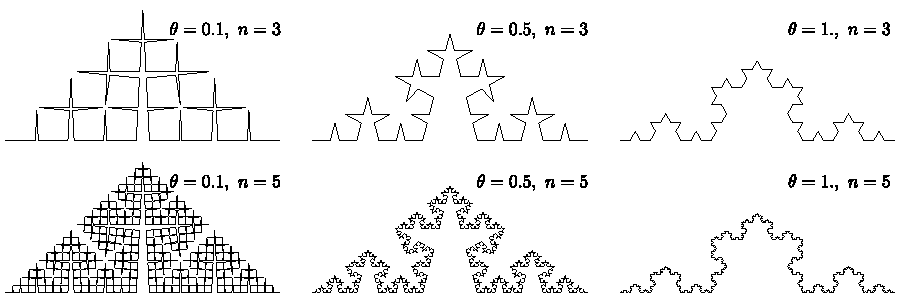
\includegraphics[width=0.7\textwidth]{figures/koch_line.pdf}
    \caption{Кривая из Т22 при разных параметрах $\theta, n$}
    \label{fig:koch}
\end{figure}
Для начала поймём, что на $n$-ном шаге всего будет $N = 4^n$ звеньев, длины $\rho$ каждый. Понятно, что
\begin{equation*}
    \sin \frac{\theta}{2} = \left(\frac{\rho_n - 2 \rho_{n+1}}{2}\right) \bigg/ \rho = \frac{\rho_n}{2 \rho_{n+1}} - 1,
    \hspace{0.5cm} \Rightarrow \hspace{0.5cm}
    \rho_n = \frac{\rho_0}{\left[
        2 +2 \sin(\theta/2)
    \right]^n}.
\end{equation*}
Длину кривой мы можем найти, как $N(\varepsilon)$ отрезков длины $\varepsilon = \rho$, тогда искомая размерность кривой
\begin{equation*}
    \textnormal{dim}(\theta) = \lim_{n \to \infty} \frac{
    \ln N(\varepsilon)
    }{
    \ln(1/\varepsilon)
    } = \lim_{n \to \infty} 
    \frac{\ln 4^n}{\ln\left[2(1+\sin \theta/2)\right]^n} = \frac{\ln 4}{\ln 2 + \ln \left[1+\sin \frac{\theta}{2}\right]},
\end{equation*}
что любопытно рассмотреть на некоторых частных случаях. 

В частности, что также видно из построения, при $\theta = 0$ кривая превратиться в некоторое покрытие плоскости умельчающейся сеткой, и $\textnormal{dim}(\theta=0) = 2$.
При $\theta = \pi/3$ мы придём к кривой Коха, с размерностью $\textnormal{dim}(\theta= \pi/3) = \ln 4/ \ln 3 \approx 1.26$, рисунок которой приведен посередине \eqref{fig:koch}. 
Наконец, при $\theta = \pi$ мы после каждой итерации будем получать прямую, и $\textnormal{dim}(\theta= \pi) = 1$. 

В случае, если мы будем говорить о размерности фигуры под рассматриваемой кривой, то обнаружим, что площадь на $n$-ной итерации может быть найдена, как
\begin{equation*}
    S_n = \frac{1}{2} \rho_0^2 \sin \theta \left[
        \frac{1}{4^2} + \frac{1}{4^3} + \ldots + \frac{1}{4^{n}}
    \right],
    \hspace{10 mm} 
    \lim_{n \to \infty} S_n = \frac{1}{24} \rho_0^2 \sin \theta,
\end{equation*}
таким образом нас интересует размерность плоской фигуры конечной площади, $N(\varepsilon) \sim \varepsilon^{-2}$ $\Rightarrow$ $\textnormal{dim} = 2$.

